\documentclass[11pt]{article}

\usepackage[T1]{fontenc}
\usepackage[utf8]{inputenc}
\IfFileExists{lmodern.sty}{\usepackage{lmodern}}{}
\usepackage[margin=1in]{geometry}
\usepackage[expansion=false]{microtype}
\usepackage{amsmath,amssymb}
\usepackage{graphicx}
\usepackage{booktabs}
\usepackage{multirow}
\usepackage{xcolor}
\usepackage{enumitem}
\usepackage[font=small,labelfont=bf]{caption}
\usepackage[round,authoryear]{natbib}
\usepackage[colorlinks=true,linkcolor=blue!60!black,citecolor=blue!60!black,urlcolor=blue!60!black]{hyperref}
\usepackage[nameinlink,capitalize]{cleveref}

% Floats stay near the text that discusses them; a barrier fires at each \section.
\usepackage[section]{placeins}
\renewcommand{\topfraction}{0.92}
\renewcommand{\bottomfraction}{0.55}
\renewcommand{\textfraction}{0.05}
\renewcommand{\floatpagefraction}{0.88}
\setcounter{topnumber}{3}
\setcounter{bottomnumber}{2}
\setcounter{totalnumber}{5}
\setlength{\floatsep}{10pt plus 2pt}
\setlength{\textfloatsep}{12pt plus 3pt}

\graphicspath{{figures/pdf/}}

% Every unknown or unfilled item is an explicit red flag.
\newcommand{\todo}[1]{\textcolor{red}{\textbf{[#1]}}}
\newcommand{\sys}{\textcolor{red}{\textbf{[SYSTEM-NAME]}}}
% A figure that no longer matches the implemented system: red note under the float, for a remake.
\newcommand{\stalefig}[1]{\par\vspace{2pt}\noindent{\footnotesize\textcolor{red}{\textbf{STALE FIGURE --- remake needed:} #1}}}
\newcommand{\mechSeed}{24}
\newcommand{\mechSigma}{0.45}
\newcommand{\mechNoFixScore}{0.85}
\newcommand{\mechChalScore}{0.99}
\newcommand{\mechProbeScore}{1.00}
\newcommand{\mechNChal}{5}
\newcommand{\mechPcTrue}{0.18}
\newcommand{\mechPcEye}{0.31}
\newcommand{\mechPcErr}{+72}
\newcommand{\mechNbTrue}{0.46}
\newcommand{\mechNbEye}{0.26}
\newcommand{\mechNbErr}{-44}
\newcommand{\mechRoundsNoFix}{12}
\newcommand{\mechRoundsChal}{15}
\newcommand{\mechRoundsProbe}{17}
\newcommand{\loopSeed}{11}
\newcommand{\loopLooks}{1}
\newcommand{\loopChal}{4}
\newcommand{\loopRounds}{12}
\newcommand{\loopReplans}{2}
\newcommand{\loopAmendRound}{3}
\newcommand{\loopRej}{6}
\newcommand{\loopInf}{2}
\newcommand{\loopTasks}{16}
\newcommand{\credBase}{0.85}
\newcommand{\credGain}{0.15}
\newcommand{\credEmpty}{0.575}
\newcommand{\hindTasks}{16}
\newcommand{\hindDropped}{heavy\_bottom}
\newcommand{\tokOld}{6.1}
\newcommand{\tokNew}{13.5}
\newcommand{\rankOld}{5}
\newcommand{\rankNew}{4}
\newcommand{\nHarnessFiles}{19}
\newcommand{\nMsgTypes}{13}
\newcommand{\nTools}{5}
\newcommand{\fxN}{80}
\newcommand{\toolSeed}{12}


\title{\textbf{Certify the Arms First: Compliant Two-Arm Teams,\\
Hosted Multi-Turn Data, and an Attributable Benchmark}\\[2pt]
{\normalsize\todo{working title: confirm}}}

\author{%
  First Author\thanks{\todo{placeholder names: replace with the real authors, affiliations and corresponding author}}
  \quad Second Author
  \quad Third Author\\[4pt]
  \todo{affiliations}
}
\date{\todo{submission date and venue (template and page limit not yet chosen)}}

\begin{document}
\maketitle

\begin{abstract}
We study a two-arm kitchen-packing team built around a single ordering constraint: the arms are certified before any language-model data generation.
Two Franka Research 3 arms run a 1\,kHz Cartesian impedance controller with a compliance supervisor that turns an external push into push, yield, bounded return and plan resume; one Qwen3.5-4B vision-language \emph{Brain} emits only skills and eye commands, never joints, stiffness or speeds.
Two movable eyes on a ring expose a rendered view library and a tool surface, and the scene bundle pairs SimReady USD assets with measured arm outcome tables.
Because hosted Kaggle tasks are CPU-only, multi-turn frontier-model episodes run against that bundle: every turn is captured, replay-verified through the same code path, and written to a success/failure memory and a per-model ledger; only certified-arm records are eligible for supervised fine-tuning.
We then train with SFT and GRPO at $k=4$ and $k=8$ and evaluate on the held-out matrix M1--M8 spanning base, trained and frontier models, zero-shot and in the harness.
Interface separation also makes failures attributable, suggesting two training signals --- counterfactual Eye credit, which replays an episode with one Eye's report replaced under common random numbers, and team hindsight relabeling, which turns failed episodes into validated records --- and we audit the upstream VIKI-Bench level~2 scorer, showing on a synthetic case that its random draw of start positions can make a score depend on luck.
This version reports the architecture, the gates and the evaluation protocol with explicit evidence classes: no task-success, benchmark, hardware or human-safety result is claimed.
\todo{The certification gates A1--A10 and the data-generation gates DG-1--DG-5 have not run; no frontier model has been called, and no trained model or benchmark row exists. Hardware safety sign-off is a separate future track (D-22).}
\end{abstract}

\section{Introduction}\label{sec:intro}

A team of language-model agents that packs a bag with two robot arms can fail for at least three different reasons.
A computer-vision Eye may misjudge what is on the table, a planner may order the packing wrongly, or an arm may drop or crush an item.
When the only recorded outcome is \emph{the bag is wrong}, these causes are indistinguishable, and so is the training signal that follows: a reward for the whole team cannot say which agent to improve.
Prior work on language-model robot teams shows that dialogue and modular agents can coordinate arms and embodied agents \citep{mandi2024roco,zhang2024coela}, and a recent benchmark and reinforcement-learning recipe for vision-language embodied cooperation \citep{kang2025vikir} makes the multi-agent setting measurable.
What these systems leave open is attribution: where in the team a failure entered, and how to turn that answer into training data.

\Cref{fig:mechanism} shows the problem on one recorded episode.
The Eye reports the pencil case as \mechPcEye{}\,kg when it weighs \mechPcTrue{}\,kg (\mechPcErr\%) and the notebook as \mechNbEye{}\,kg when it weighs \mechNbTrue{}\,kg (\mechNbErr\%).
The Brain, reasoning correctly from those numbers, stacks the heavier notebook on the lighter pencil case; the team breaks the rule that heavy items go at the bottom and scores \mechNoFixScore{}.
The error is the Eye's, but the failure surfaces in the plan and is only visible in the final bag.
Two mechanisms repair it: an Arm that weighs the item in its gripper can challenge the Eye, and the Arms can weigh every item before planning.
Both are cheap to state and easy to test in a symbolic world, which is why we build the team around interfaces where such evidence can be exchanged.

\begin{figure*}[tbp]
\centering
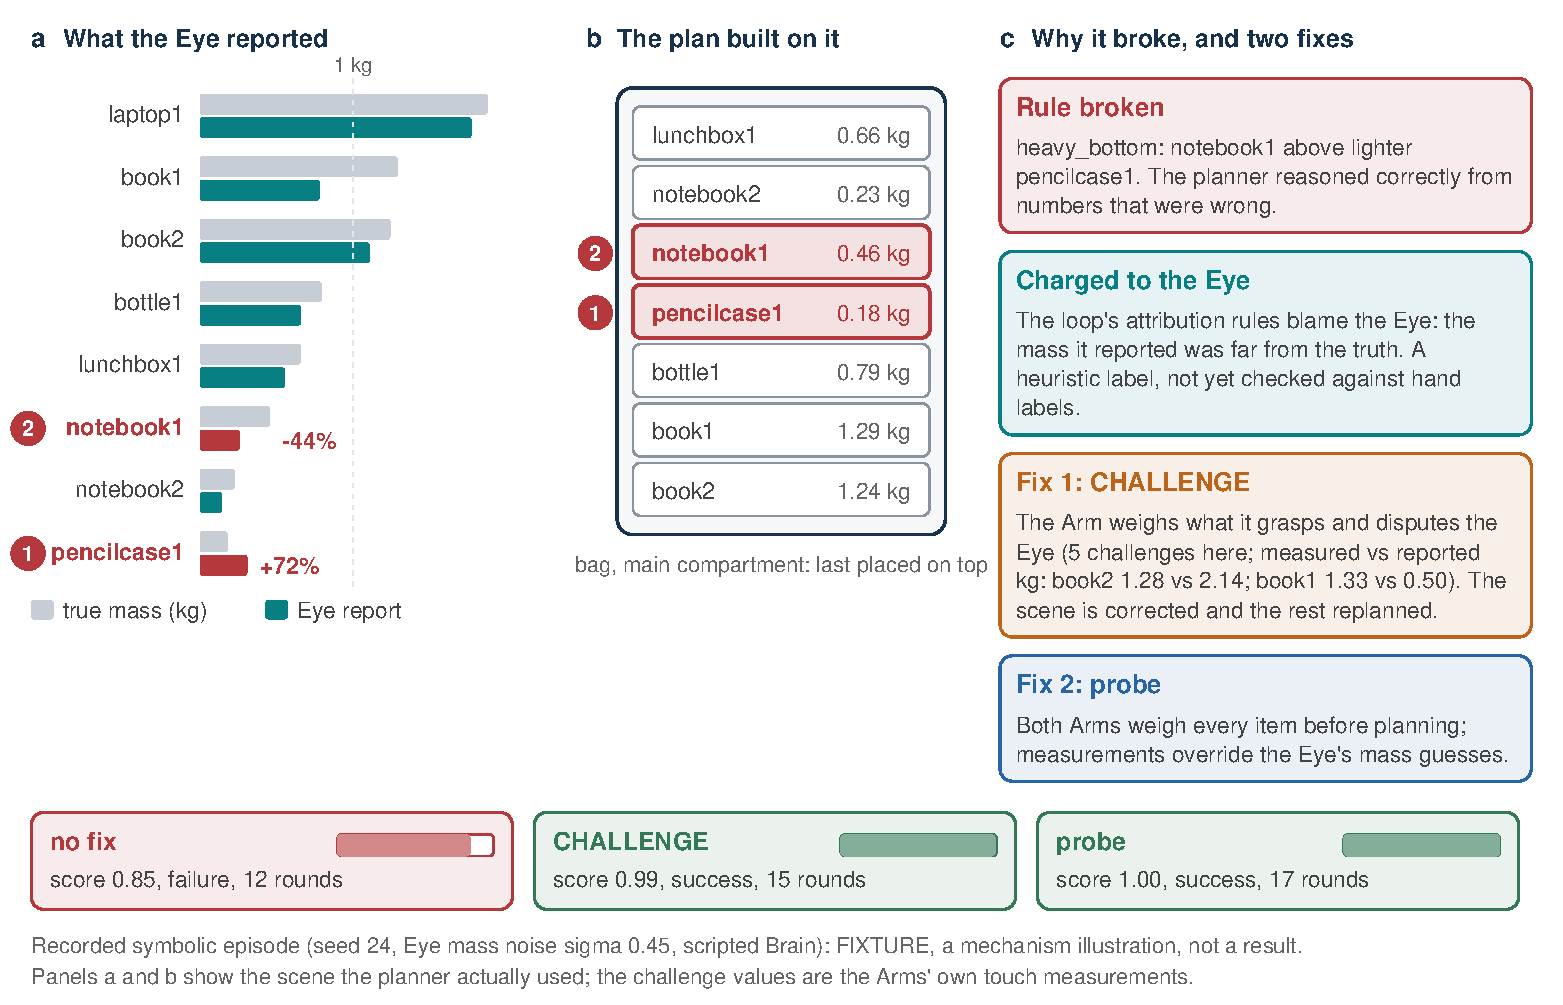
\includegraphics[width=\textwidth]{fig_mechanism}
\caption{\textbf{The problem and our approach (schematic).} (1)~A team of Eyes, a Brain and Arms packs items. Here a heavier item ends up on a lighter one and only one team reward is observed, so it is unclear which agent should learn; typed messages (SCENE, PLAN) make each agent's claims checkable. (2)~We replay the failed episode once per agent, with that agent's contribution replaced by an oracle and all random draws shared; the agent whose replacement repairs the episode carries the responsibility. (3)~Responsibility routes learning: the Eye is updated by credit-guided rejection sampling, the Brain receives the failed episode back as a relabeled, replay-checked example, and an agent that was not to blame is left unchanged. The Eye replay is measured on a recorded fixture episode (seed \mechSeed{}); the Brain and Arm oracle replays drawn here are what the design predicts for that failure and are not yet implemented. Icons are pictograms, not rendered images.}
\label{fig:mechanism}
\end{figure*}

We design the team so that this tracing is possible by construction (\cref{fig:overview}).
\emph{Roles are separated by interface}: only the Eyes receive pixels, only the Brain plans, and the Arms are blind executors that report force and touch.
All communication is a typed, budgeted message (\cref{sec:bus}), so every claim an agent makes about the scene can be compared with what another agent later observes.
The Brain works from a small file-based harness and can check a plan with a deterministic dry run before anything moves (\cref{sec:harness,sec:tools}).
Because the roles are separate, two training signals become natural: replaying an episode with one Eye's report replaced estimates how much that Eye cost the team, and finished episodes, including failed ones, can be relabeled with what the team actually achieved (\cref{sec:signals}).
A single success checker scores the symbolic world and a pose-level simulator and is designed to extend to Isaac Lab (\cref{sec:bridge}), so that a claim made in the cheap world can eventually be re-tested under physics \todo{only the Newton rgb/depth stepping gate G-3 is measured; the manipulation scene and its checker do not exist}.

\paragraph{Contributions.}
\begin{enumerate}[leftmargin=*,itemsep=1pt]
\item A role-separated team design with typed messages, a harness and verification tools in which each failure has an interface to blame (\cref{sec:method}).
\item Two learning signals, counterfactual Eye credit under common random numbers and team hindsight relabeling with a replay check, specified with their assumptions (\cref{sec:signals}).
\item One success definition shared by a symbolic world and a pose-level simulator, designed to extend to Isaac Lab, so plan validity and physical success can be compared \todo{only the gate is measured; no Isaac Lab manipulation result} (\cref{sec:bridge}).
\item An audit of the upstream VIKI-Bench level-2 scorer with a synthetic demonstration, and an evaluation protocol that separates evidence classes (\cref{sec:experiments}).
\end{enumerate}

\paragraph{Status of the evidence.}
This version contains no reportable task-success, benchmark or comparison result.
The system is implemented and its wiring is tested. Gates G-1, G-2, G-3 and G-14 record \emph{engineering} measurements on the real stack --- the Qwen3.5 module map, the DeltaNet fast path, Newton-only rgb/depth stepping on both an RTX 4050 and a Kaggle T4 (a falling cube, stepped on one of the two available devices at a time), and a four-step QLoRA run that resumes mid-epoch from a checkpoint fetched from our private repository; the last is a smoke test, not a trained model. Gate G-6 adds a \emph{simulation-only} impedance cross-check (analytic step error 0.27\,\%, with a push and return measured), not a safety certification. These gates establish that the pipeline runs; they are not evidence about packing performance.
The mechanism figures and appendix~F come from a symbolic fixture with a scripted Brain and parametric Eyes (evidence class FIXTURE), which checks that mechanisms work and says nothing about trained agents.
\todo{Pending, with no report: SimReady asset ingestion and an asset-based kitchen scene; frontier-model CoT (\texttt{RTP\_SERVE\_URL} unset, scripted teacher traces only); training on environment episodes; a fixed held-out test set; omni-model scores; and impedance control on hardware. G-14 is a smoke, not a model-quality result.}
Every unfilled number is a red flag and a row in a machine-readable pending list; \cref{tab:evidence} states the status of each evidence class.

\section{Related work}\label{sec:related}

\paragraph{Cooperative embodied agents with language models.}
VIKI-R \citep{kang2025vikir} introduces VIKI-Bench, a hierarchical benchmark for embodied multi-agent cooperation with vision-language models, and a two-stage recipe of supervised fine-tuning followed by reinforcement learning; it is our starting point, and \cref{sec:track-a} reuses its released data and checkpoints.
RoCo \citep{mandi2024roco} has language-model agents, one per robot arm, discuss and agree a plan that is grounded by motion planning.
CoELA \citep{zhang2024coela} builds embodied agents from separate perception, memory, communication, planning and execution modules around a language model.
Our work differs in emphasis: we fix the roles by interface, so that a failure has an owner, and we treat the team's own failures as the source of training signal.
\todo{Related work to read and add before submission: further multi-agent embodied and robot-team papers (the plan names CHORUS, D-VLC, MAAP, C3/CCPO and others by name only; none has been opened yet, so none is cited or compared).}

\paragraph{Credit assignment and hindsight.}
Hindsight experience replay \citep{andrychowicz2017her} relabels a failed attempt with the goal it did reach; our team hindsight relabeling applies the idea to instructions and adds a replay check (\cref{sec:signals}).
Counterfactual baselines for multi-agent credit \citep{foerster2018coma} replace one agent's action and compare returns; our Eye credit replaces one Eye's \emph{report} and replays the whole episode.
\todo{Confirm and cite the difference-rewards literature if it is kept in the final text.}

\paragraph{Training signals and simulation.}
We use group-relative policy optimization \citep{shao2024deepseekmath} for the Brain, flow matching \citep{lipman2023flowmatching} for the Arm policy, low-rank adaptation \citep{hu2022lora} for the language and vision models, and Isaac Lab \citep{mittal2025isaaclab} for physics. \todo{Citations marked TODO-verify in \texttt{refs.bib}: confirm each against its source before submission.}

\paragraph{Benchmark scoring.}
A level-2 plan is scored by a simulator-free checker in the upstream VIKI-R repository; we read that code and report an audit in \cref{sec:scorer}.
\todo{LOCUS-Bench, a derived benchmark, was only available as an anonymized review artifact marked not for redistribution; it is neither cited nor compared. Revisit if it becomes public.}

\section{The team}\label{sec:method}

\begin{figure*}[tbp]
\centering
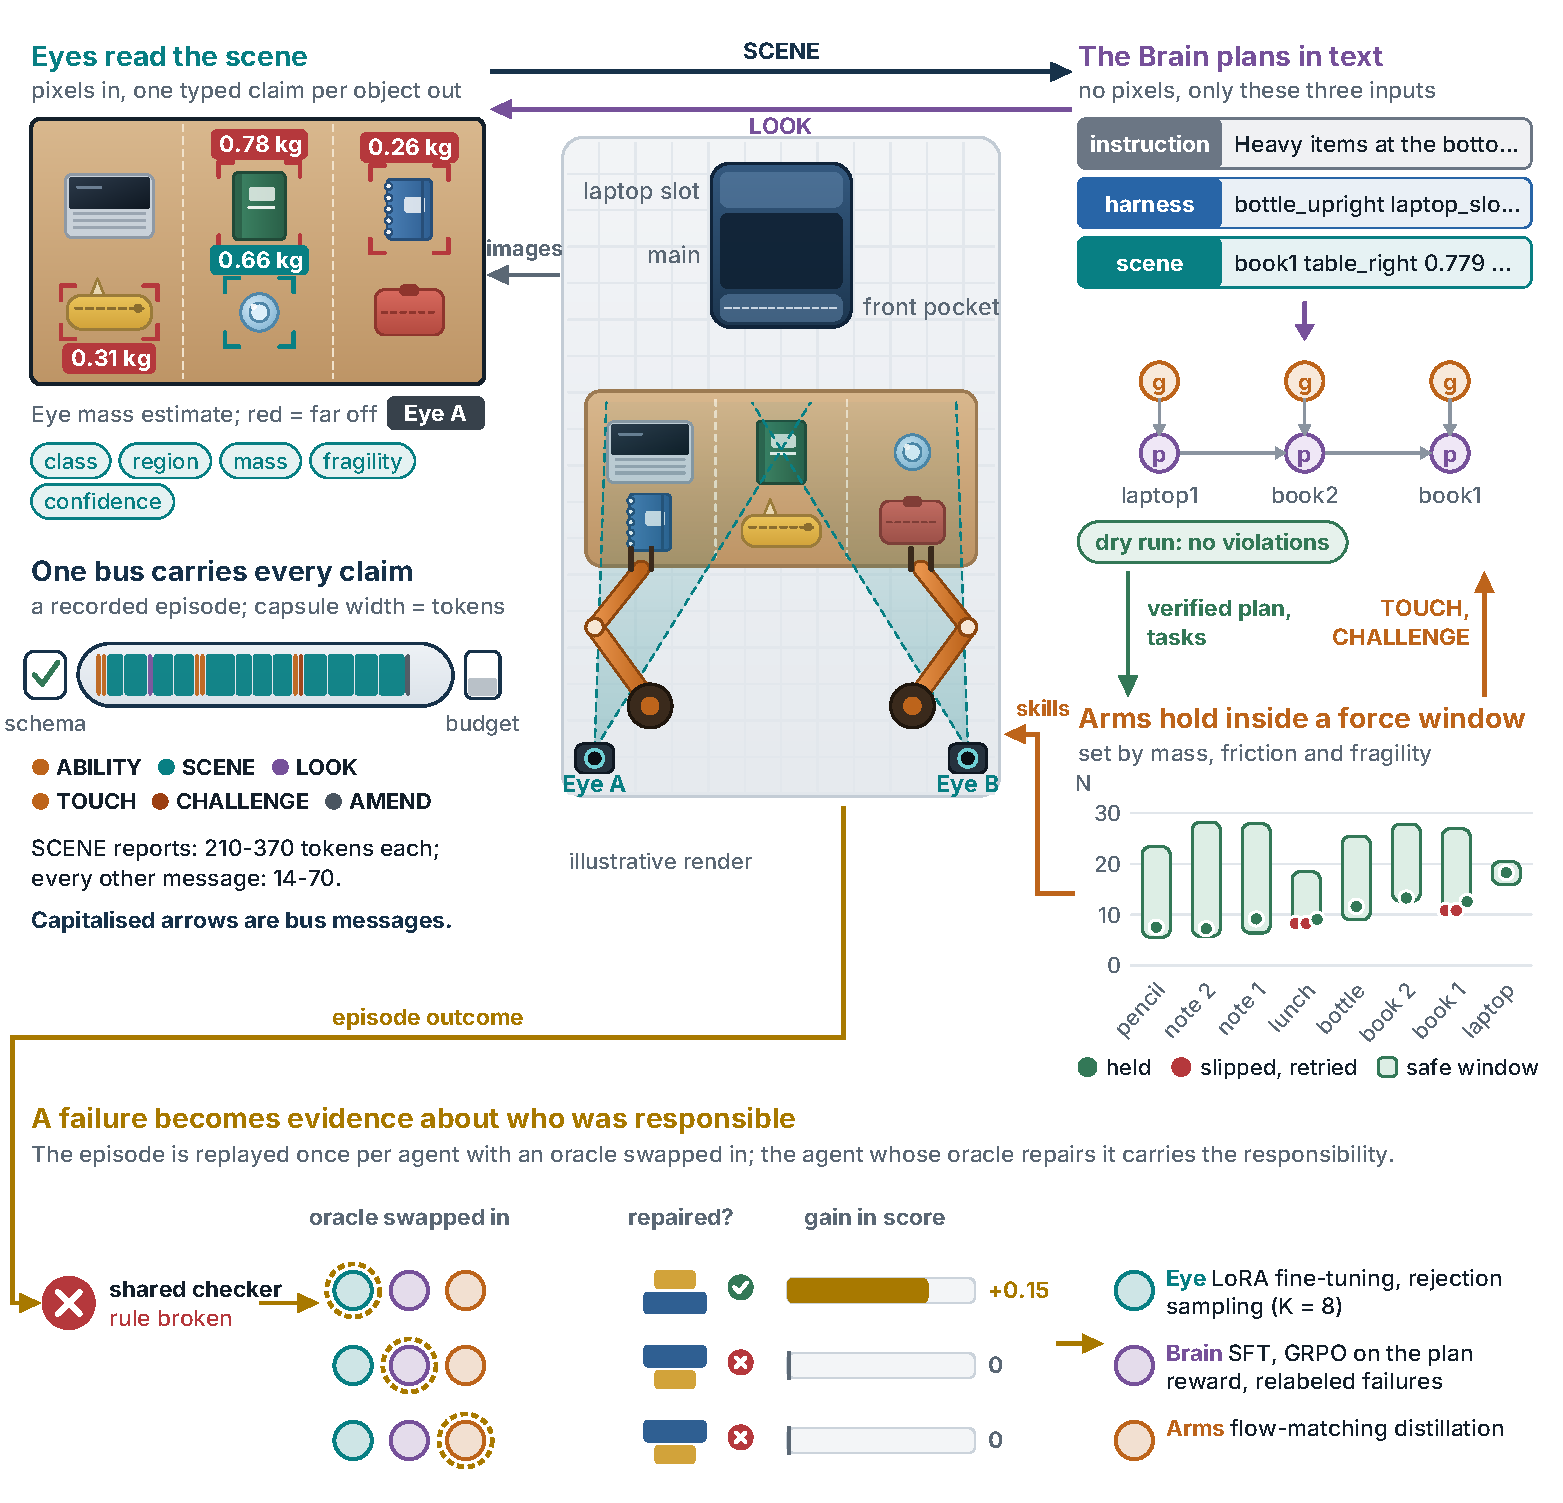
\includegraphics[width=0.92\textwidth]{fig_overview}
\caption{\textbf{The team and its interfaces.} Eyes see pixels and emit a structured scene; the Brain reads text, retrieves from the harness, and plans; a verifier checks the plan before the scheduler hands tasks to two blind Arms; touch and challenges flow back through a typed message bus. Numbers give the order of one episode. Dashed boxes are optional; red tags mark components whose trained models do not yet exist.}
\label{fig:overview}
\end{figure*}

\subsection{Task, roles and failure model}\label{sec:task}
The task is to pack a backpack from a table: given a short natural-language instruction (for example which items to pack and which rules to respect), two arms must place the requested items into the bag's compartments.
The six rules are in \cref{tab:rules}: heavier items go first so that they sit at the bottom of the main compartment, the laptop goes in its slot, the bottle stays upright and apart from the laptop, the lunchbox goes in last, distractor items are left alone, and only one arm may be at the bag at a time.
The team has three kinds of agents (\cref{fig:overview}).
Each \emph{Eye} is a vision-language model that sees an image and emits a JSON scene listing each object's class, region, estimated mass and fragility.
The \emph{Brain} is a text-only language model; it never sees pixels and plans a directed acyclic graph of grasp and place tasks.
Each \emph{Arm} is blind: it has proprioception, force sensing and a skill interface, and reports what it feels.
Failures are charged to an agent by the loop's attribution rules (\cref{sec:success}); these are heuristic labels, which we validate in \cref{sec:experiments}.

\begin{table}[tbp]
\centering\small
\begin{tabular}{lp{0.74\linewidth}}
\toprule
Rule file & Text given to the Brain (verbatim from the harness file) \\
\midrule
\texttt{bag\_exclusive} & Only one arm may place into the bag at a time. Serialize place tasks with dependencies. \\
\texttt{bottle\_upright} & Water bottles go in upright and in a different compartment from the laptop. Use orientation=upright. \\
\texttt{heavy\_bottom} & Place heavier items first so they sit at the bottom of the main compartment; lighter items go on top. Sort items by estimated mass, descending. \\
\texttt{laptop\_slot} & The laptop goes in the compartment named by the instruction (default: the padded laptop slot). Never stack other items on or beside it in the same compartment. \\
\texttt{leave\_distractors} & Items the instruction says to leave (for example the mug and the plate) must not be touched, moved or pushed aside. \\
\texttt{lunchbox\_last} & The lunchbox is packed last so it sits on top and stays accessible. \\
\bottomrule
\end{tabular}

\caption{The six rules the team must satisfy; the text is the harness file the Brain retrieves (\cref{sec:harness}).}
\label{tab:rules}
\end{table}

\subsection{Typed messages}\label{sec:bus}
Agents exchange \nMsgTypes{} message types (\cref{fig:messages}, \cref{tab:messages}): scene reports, ability declarations, task claims and offers, status and blockage notices, touch feedback, requests to look again, challenges, handovers, locks and amendments of the instruction.
The bus checks each message against its schema, charges an approximate token count (about four characters per token, a tokenizer-free proxy) and enforces a per-episode budget; an over-budget message is refused and the sender is told.
We implement four communication modes: \emph{push} sends the full scene every round, \emph{delta} sends only changed objects, \emph{pull} sends on request and after failures, and \emph{init-only} sends once.
The modes trade tokens for information, and their effect on trained agents is a pending ablation (\cref{tab:ablations}); the accounting itself is checked on the fixture in appendix~F.

\begin{figure*}[tbp]
\centering
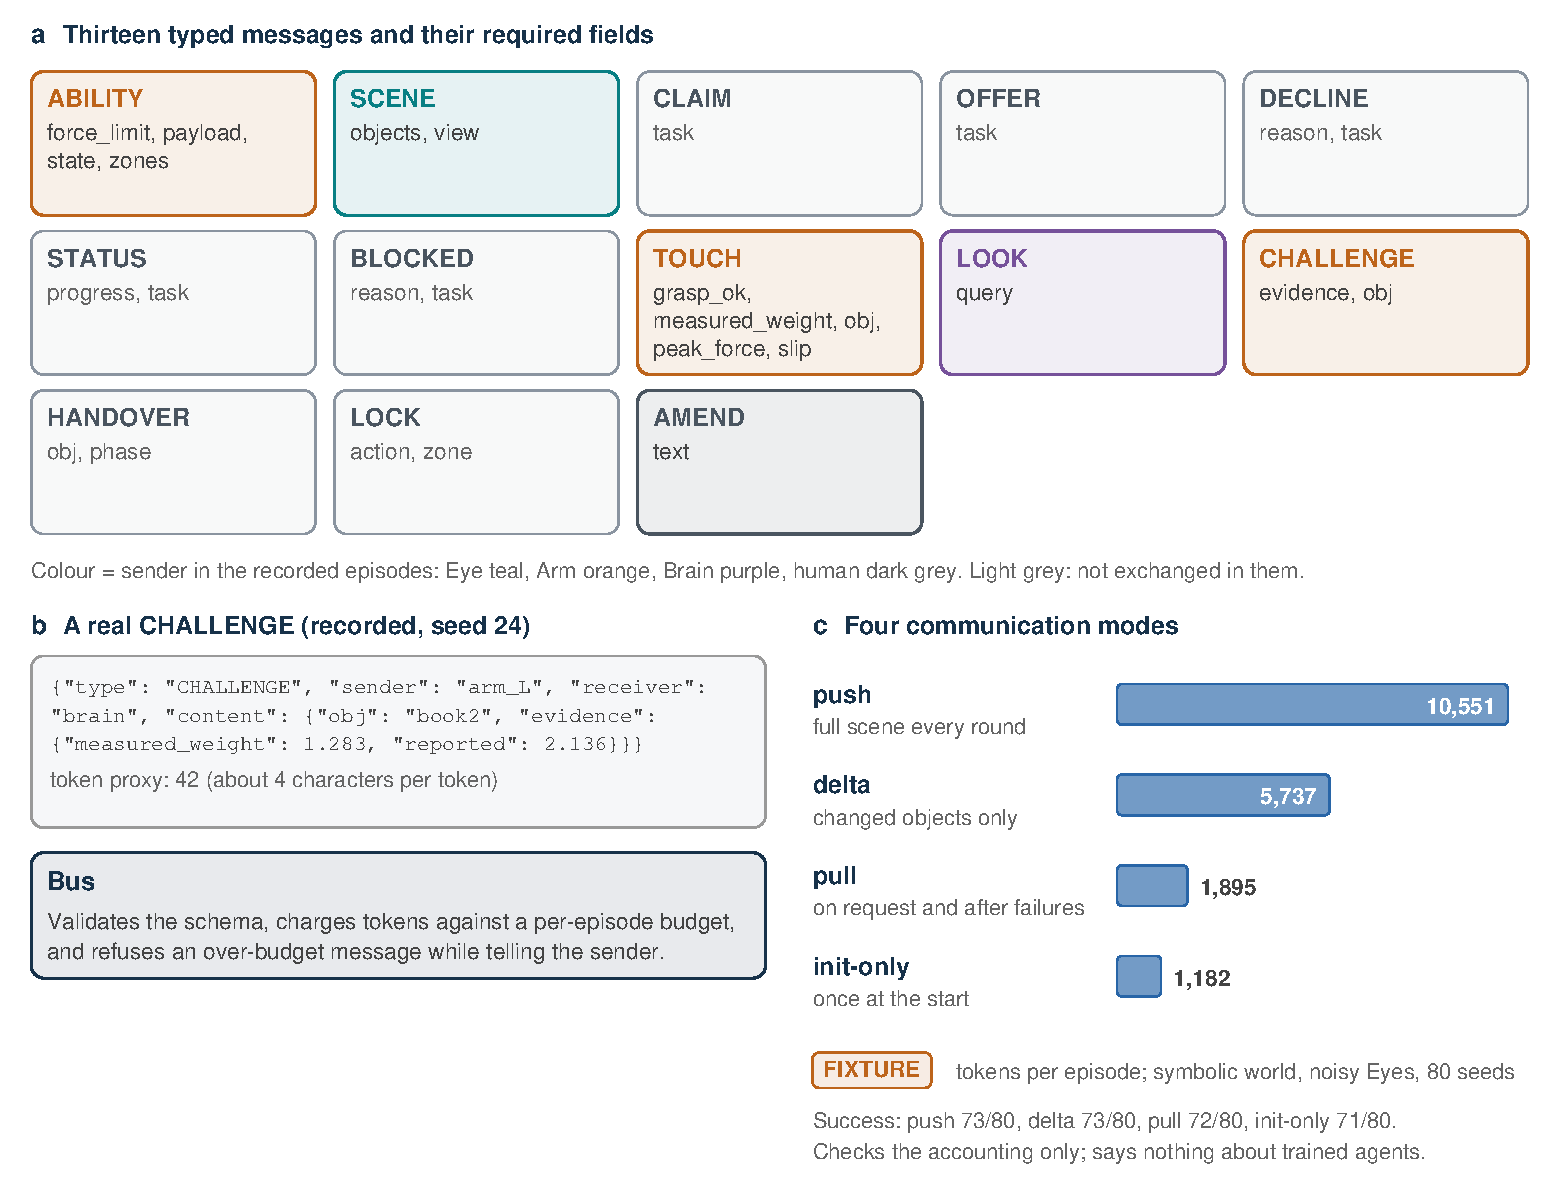
\includegraphics[width=\textwidth]{fig_messages}
\caption{\textbf{The message layer.} (a)~The \nMsgTypes{} types and their required fields; colour shows the sender observed in the recorded episodes. (b)~A recorded CHALLENGE: an Arm reports a measured weight that disagrees with the Eye's report. (c)~Message tokens per episode under four communication modes, from the symbolic fixture (80 seeds): a check that the accounting works, not a result about trained agents.}
\label{fig:messages}
\end{figure*}

\begin{table}[tbp]
\centering\scriptsize
\begin{tabular}{lp{0.38\linewidth}p{0.3\linewidth}}
\toprule
Type & Required fields & Sender in the recorded episode \\
\midrule
\texttt{ABILITY} & force\_limit, payload, state, zones & arm \\
\texttt{SCENE} & objects, view & eye \\
\texttt{CLAIM} & task & not exchanged in the recorded episode \\
\texttt{OFFER} & task & not exchanged in the recorded episode \\
\texttt{DECLINE} & reason, task & not exchanged in the recorded episode \\
\texttt{STATUS} & progress, task & not exchanged in the recorded episode \\
\texttt{BLOCKED} & reason, task & not exchanged in the recorded episode \\
\texttt{TOUCH} & grasp\_ok, measured\_weight, obj, peak\_force, slip & arm \\
\texttt{LOOK} & query & brain \\
\texttt{CHALLENGE} & evidence, obj & arm \\
\texttt{HANDOVER} & obj, phase & not exchanged in the recorded episode \\
\texttt{LOCK} & action, zone & not exchanged in the recorded episode \\
\texttt{AMEND} & text & human \\
\bottomrule
\end{tabular}

\caption{Message schema as implemented. The sender column lists what was observed in the recorded episode of \cref{fig:loop}; it is not a constraint of the schema.}
\label{tab:messages}
\end{table}

\subsection{The harness}\label{sec:harness}
The Brain's procedural knowledge lives in \nHarnessFiles{} short markdown files (\cref{fig:harness}, appendix~B): the six rules, four skill descriptions, object and agent notes, an episode memory and a task template.
Retrieval is a two-pass BM25 search.
Pass one queries with the instruction and returns the top five of the six rules; pass two queries with the classes present in the scene and returns the top three object, skill and memory notes.
The retrieved text is added to the Brain's context.
After episodes, a monitor writes measured success rates and failure causes back into the skill files.
The harness is a design choice about where knowledge lives (editable text, not weights); whether it helps a trained Brain is the pending harness ablation.

A tokenizer defect illustrates why retrieval needs its own tests.
A tokenizer that keeps alphanumeric runs together reads \texttt{lunchbox1} as one token that never matches \texttt{lunchbox} in the lunchbox rule; the fixed tokenizer splits letters from digits.
On the recorded instruction, our reconstruction of the pre-fix tokenizer scores the lunchbox rule \tokOld{} and ranks it \rankOld{}th of six, just above a rule that is not required; the fixed tokenizer scores it \tokNew{} and ranks it \rankNew{}th (\cref{fig:harness}c).
At five retrieved rules both retrieve every required rule for this instruction, so the fix widens a margin here; we do not reproduce the earlier case in which a required rule was dropped.

\begin{figure*}[tbp]
\centering
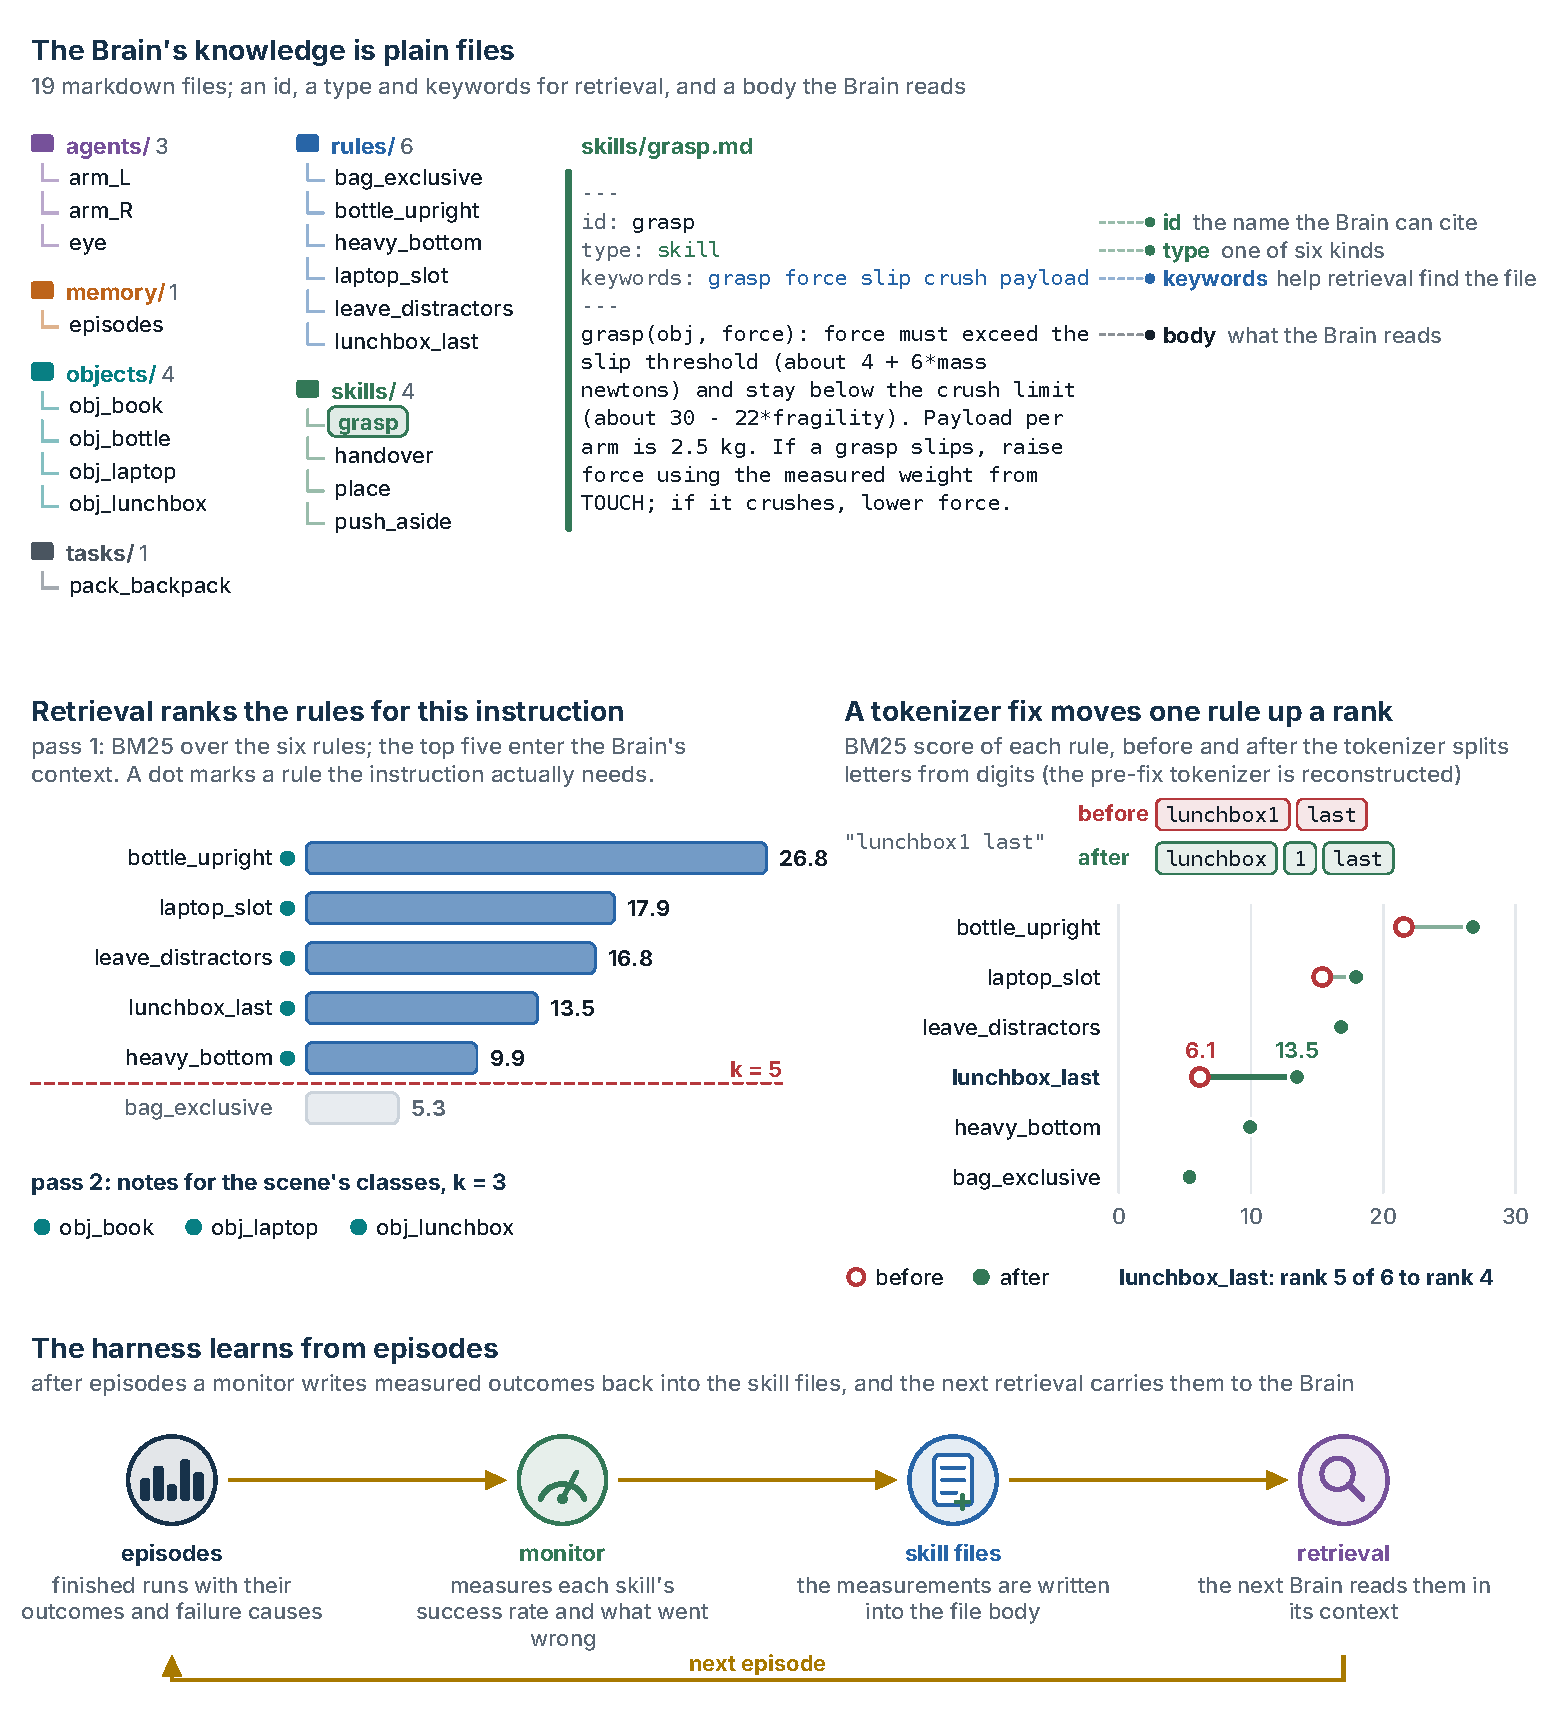
\includegraphics[width=\textwidth]{fig_harness}
\caption{\textbf{The harness.} (a)~The \nHarnessFiles{} markdown files by type. (b)~Two-pass BM25 retrieval into the Brain's context, with a monitor that writes measured outcomes back to the skill files (dashed: runs after episodes). (c)~Tokenization of the string ``lunchbox1 last'' before and after the fix, and the BM25 score of every rule for the recorded instruction. The pre-fix tokenizer is our reconstruction.}
\label{fig:harness}
\end{figure*}

\subsection{Planning with tools and verification}\label{sec:tools}
The Brain can be a plain planner or a tool-using one (\cref{fig:tools}).
The tool-using Brain has \nTools{} tools: \texttt{check\_rule}, \texttt{query\_scene}, \texttt{look}, \texttt{dry\_run} and \texttt{submit\_plan}.
\texttt{dry\_run} executes a draft plan deterministically in the symbolic world and returns the rule violations and failed tasks, which is the evidence the Brain revises against; the prompt asks it to dry-run before submitting, it has at most six turns, and replying with a bare plan also commits.
Independently of the tools, the loop can verify a plan before any arm moves: not at all, with a static feasibility check, or with a full dry run; a rejected plan is returned with the reasons for up to two retries.
We test the verifier against a flaky-planner fixture in appendix~F.

\begin{figure*}[tbp]
\centering
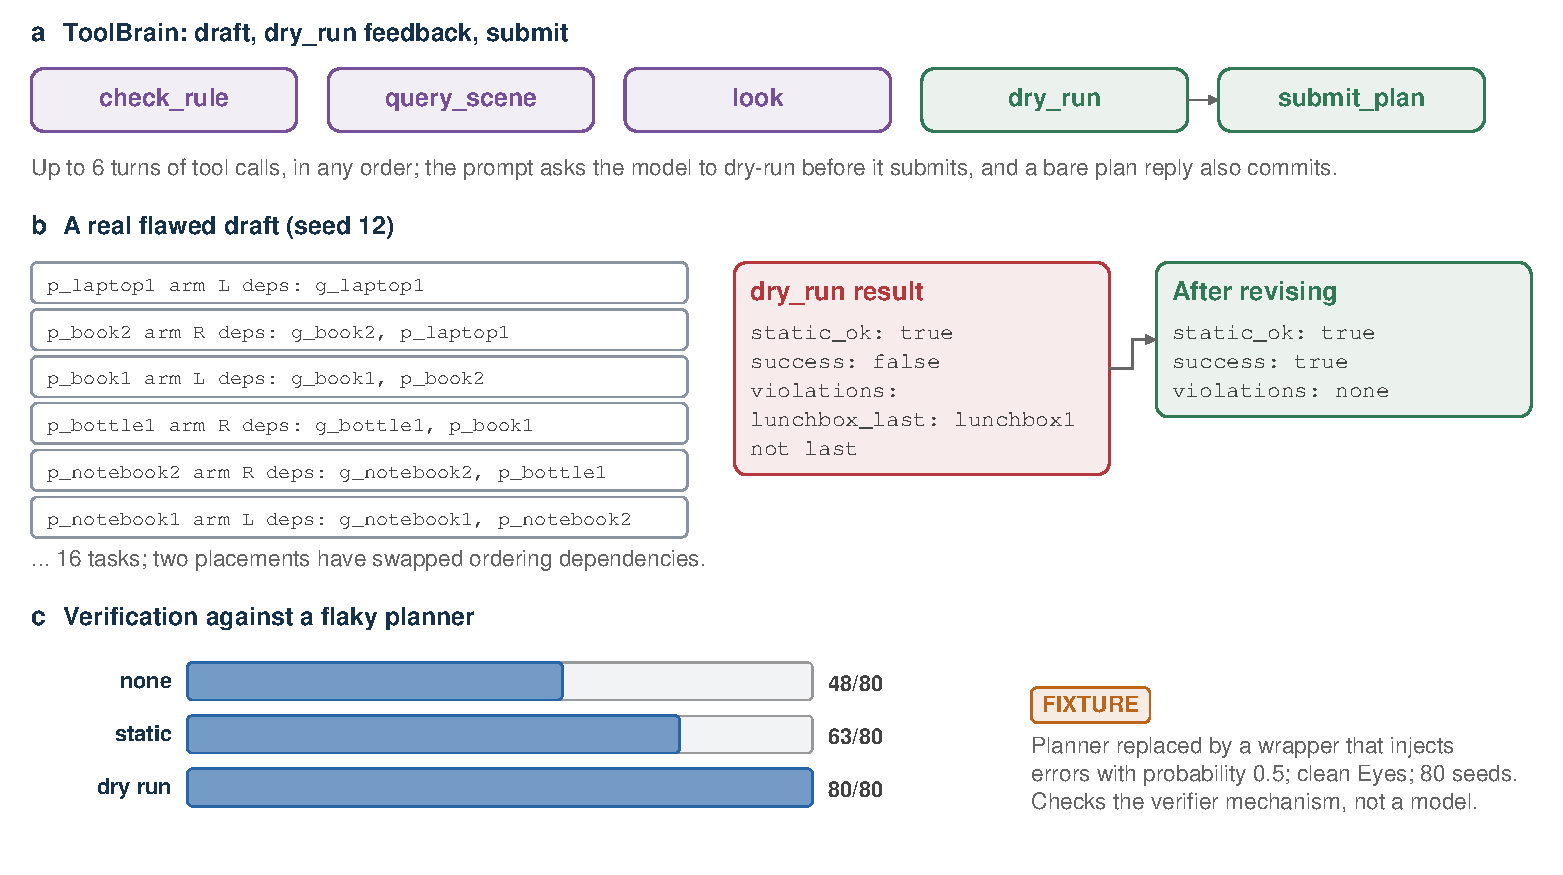
\includegraphics[width=\textwidth]{fig_tools}
\caption{\textbf{Tools and verification.} (a)~The five tools of the tool-using Brain. (b)~A recorded flawed draft (seed \toolSeed{}, two placements with swapped ordering dependencies) and the \texttt{dry\_run} feedback it receives; the revised plan passes. (c)~Verification against a planner replaced by a wrapper that injects errors with probability 0.5 (fixture, 80 seeds): a check of the verifier, not of a model.}
\label{fig:tools}
\end{figure*}

\subsection{The control loop}\label{sec:loop}
An episode runs as in \cref{fig:loop}.
The Eyes report a scene; an optional \emph{probe} has the Arms weigh every item and overrides the Eye mass guesses with measurements.
The Brain plans and the verifier checks.
If a requested item is missing from the scene, the Brain asks the Eyes to \textsc{look} again and replans.
In each round the scheduler gives each Arm its head task, with exclusive access to the bag.
When an Arm touches an item whose measured weight differs from the Eye's report by more than 20\%, it sends a \textsc{challenge}, the scene is corrected and the remaining placements are replanned once.
A human may \textsc{amend} the instruction mid-episode, which forces a replan.
A failed skill climbs a recovery ladder: retry, alternate parameters, retreat, reassign to the other Arm, replan, abort.
At the end the checker of \cref{sec:success} scores the bag and attributes fatal failures.

\begin{figure*}[tbp]
\centering
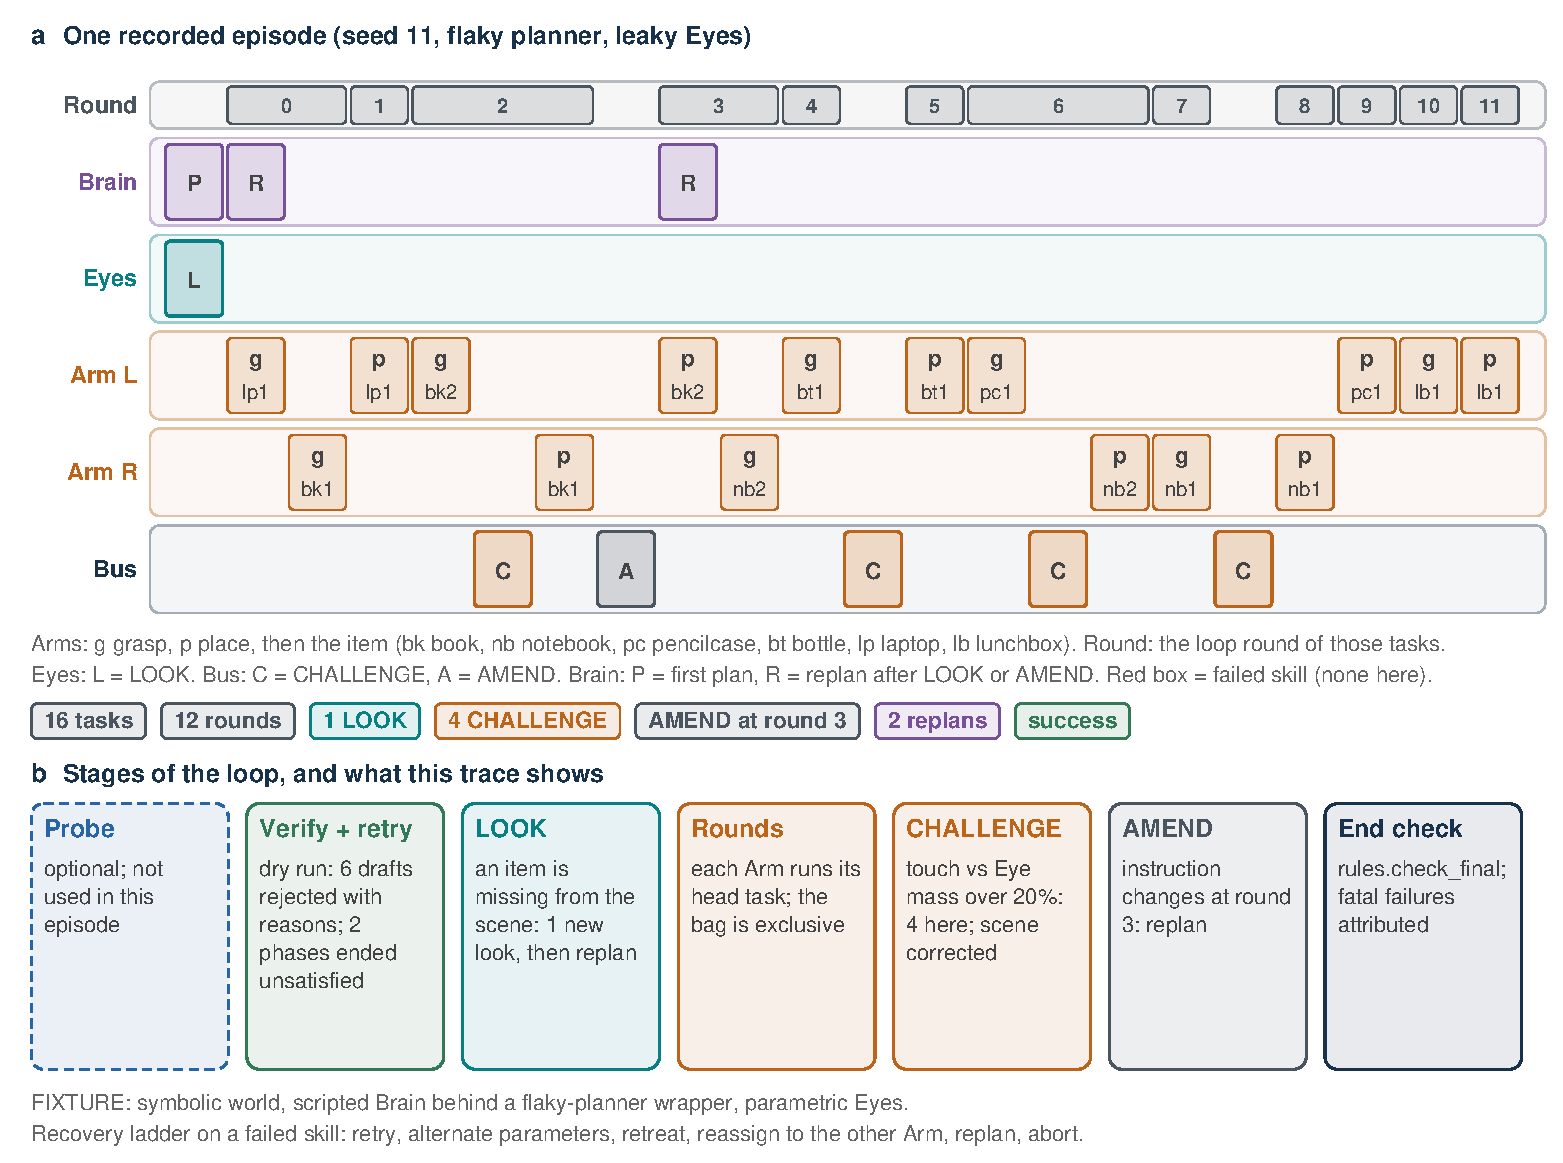
\includegraphics[width=\textwidth]{fig_loop}
\caption{\textbf{One recorded episode through the loop} (seed \loopSeed{}, flaky planner, leaky Eyes; fixture). (a)~The \loopTasks{} executed tasks by arm in time order, with the loop round of each, the \loopLooks{} look, \loopChal{} challenges, the amendment at round \loopAmendRound{} and the replans (\loopReplans{}); the episode takes \loopRounds{} rounds and succeeds. (b)~The stages of the loop and what this trace shows of each, including the planner's \loopRej{} rejected drafts; the probe is not used here.}
\label{fig:loop}
\end{figure*}

\subsection{Success, forces and attribution}\label{sec:success}
One function, \texttt{rules.check\_final}, defines success in every world: every requested item is packed, no rule is violated and nothing is crushed; the score is the valid-item fraction minus 0.15 per violation, 0.3 per crushed item and 0.01 per replan.
In the symbolic world a grasp slips when its force is below $(4+6m)/f$ newtons for mass $m$ and friction $f$, and crushes when it exceeds $30-22\,\phi$ newtons for fragility $\phi$.
Failures are attributed by rules: a slip or crush is charged to the Eye when the reported mass or fragility was off by more than 15\%, otherwise to the Arm; a rule violation is charged to the agent whose report or plan produced it.
These are heuristics; \cref{tab:attribution} is the hand-labelled check we owe the reader.

\subsection{Learning signals}\label{sec:signals}
\Cref{fig:signals} lists what trains what.
Each Eye is fine-tuned with LoRA on rendered images with scene targets and then improved by rejection sampling: $K=8$ reports per image, keeping the best by field accuracy or by counterfactual credit.
The Brain is fine-tuned on teacher plans that were validated by closed-loop success and then optimized with GRPO using a plan-level reward $R = 0.1\,r_{\text{format}} + 0.2\,r_{\text{feasible}} + 0.6\,r_{\text{rules}} + 0.1\,r_{\text{length}}$, optionally plus a closed-loop rollout term; the components are defined in \cref{fig:signals}.
The Arms are a small transformer trained by distillation of scripted differential-IK demonstrations with a flow-matching action head: with $x_t=(1-t)x_0+t\,x_1$, noise $x_0$ and action chunk $x_1$, the network predicts $x_1-x_0$; sampling uses eight Euler steps, a chunk of 16 actions of dimension 8, and executes the first four before replanning.
There is no learned stop signal, so a skill ends by a scripted completion test.

\paragraph{Counterfactual Eye credit.}
For an episode with score $R(\text{real})$, replace Eye $i$'s report by a replacement $r$ (empty, degraded or the oracle truth, optionally for one field only) and replay with the same keyed random draws, giving $R(i,r)$.
The credit is $C(i,r)=R(\text{real})-R(i,r)$, so a positive credit means the Eye helped relative to the replacement; the \emph{oracle gain} $G=R(\text{oracle})-R(\text{real})=-C(i,\text{oracle})$ is what a perfect Eye would have added.
All random draws are keyed by (seed, arm, skill, object, attempt), so replays share common random numbers.
The estimate has two caveats: it is a team counterfactual and is not additive across redundant Eyes, and with a Brain that adapts to the replaced report it measures the adapted team, not the original plan.
\Cref{fig:credit}a shows one recorded case: a perfect Eye~A would recover \credGain{} of a score of \credBase{}, all of it in the mass field.

\paragraph{Team hindsight relabeling.}
A finished episode is relabeled with what the team achieved: the instruction is rewritten to the rules that held, and the executed plan becomes the target.
The record is admitted only if replaying the executed plan from the initial state satisfies the relabeled instruction.
In \cref{fig:credit}b the failed episode of \cref{fig:mechanism} is relabeled by dropping \hindDropped{}, and its \hindTasks{}-task plan passes the replay check.
The relabeled instruction is weaker than the original, so relabeled data teaches obedience to what was achievable and must be mixed with unrelabeled data; the mixing ratio is a pending ablation.

\begin{figure}[tbp]
\centering
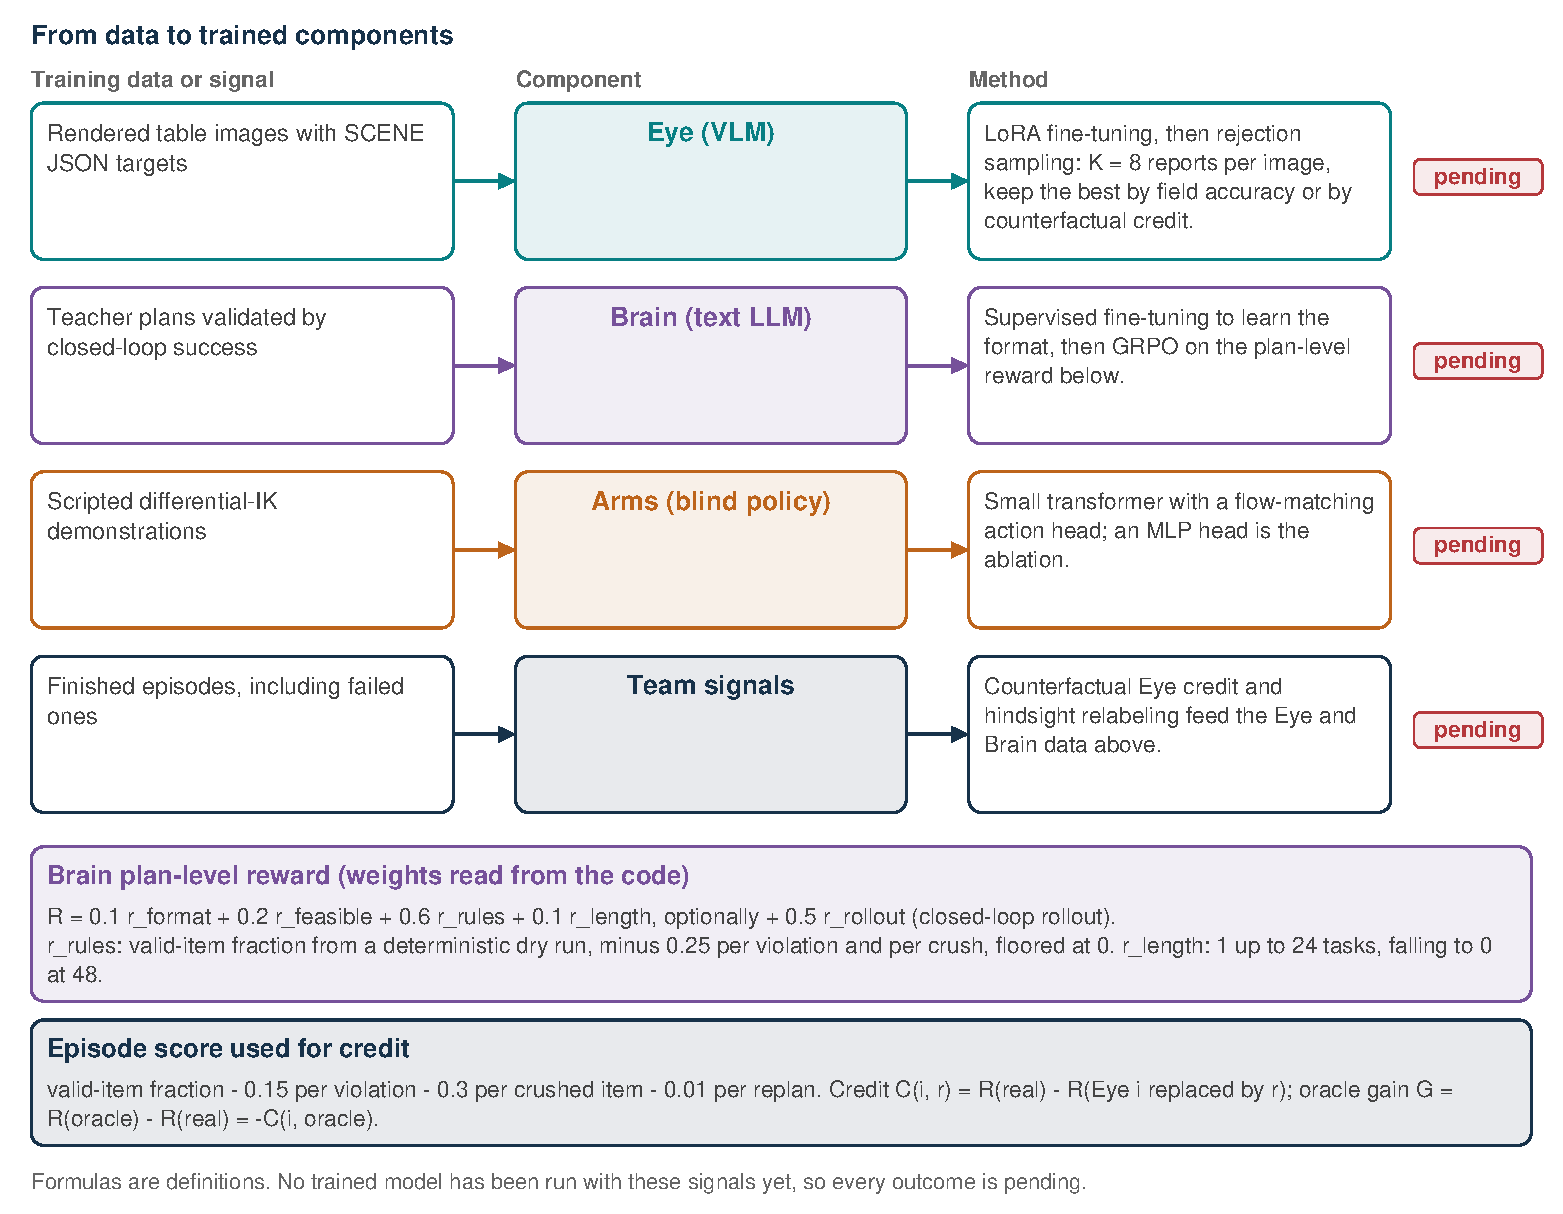
\includegraphics[width=\columnwidth]{fig_signals}
\caption{\textbf{Learning signals.} From training data through component to method, then the plan-level reward read from the code and the episode score used for credit. No trained model has been run with these signals, so all outcomes are pending.}
\label{fig:signals}
\end{figure}

\begin{figure*}[tbp]
\centering
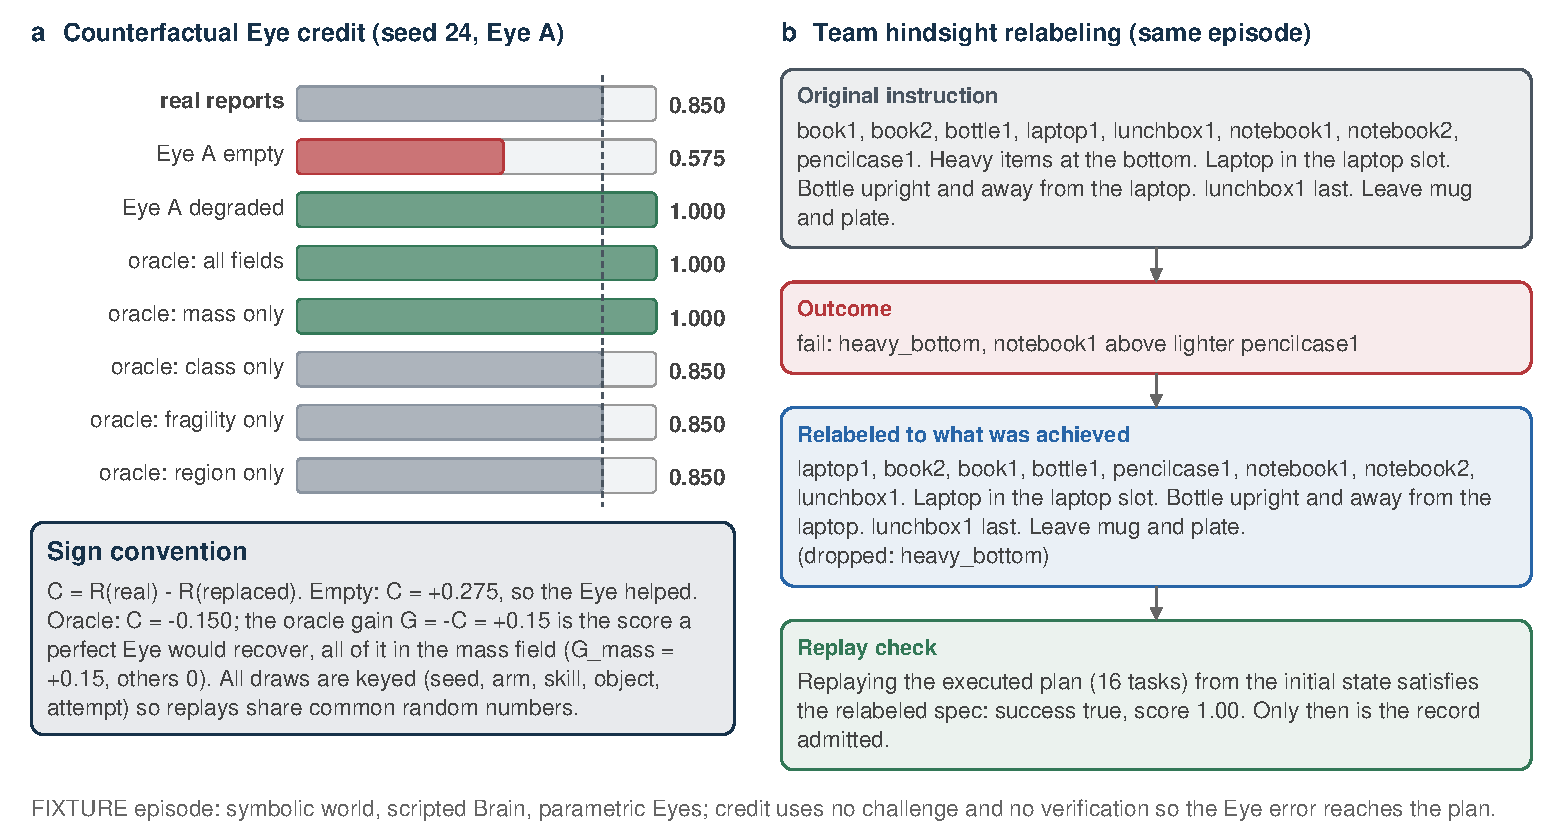
\includegraphics[width=\textwidth]{fig_credit}
\caption{\textbf{Two team-level signals on the episode of \cref{fig:mechanism}.} (a)~Counterfactual credit for Eye~A: replacing its report changes the episode score; the dashed line is the real score (\credBase{}) and an empty report would score \credEmpty{}. (b)~Hindsight relabeling: the failed episode is rewritten to what it achieved and admitted only after a replay check. Fixture episode (no challenge, no verification, so the Eye error reaches the plan).}
\label{fig:credit}
\end{figure*}

\subsection{One success definition across three worlds}\label{sec:bridge}
The same team runs in three worlds (\cref{fig:bridge}): the symbolic world, in which the loop is developed; a pose-level fake simulator that takes poses, maps them to regions and compartments through a bridge and reproduces the symbolic world's loop outcomes in tests; and Isaac Lab, where skill outcomes (success, slip, crush, out of reach, wrong slot, no space, locked, overload, not holding, hand full) are derived from the state before and after a skill.
Because \texttt{rules.check\_final} scores all three, the difference between a plan that is valid in the symbolic world and one that succeeds under physics can be measured instead of assumed.
The pose-level test validates the integration, not the physics.

\begin{figure*}[tbp]
\centering
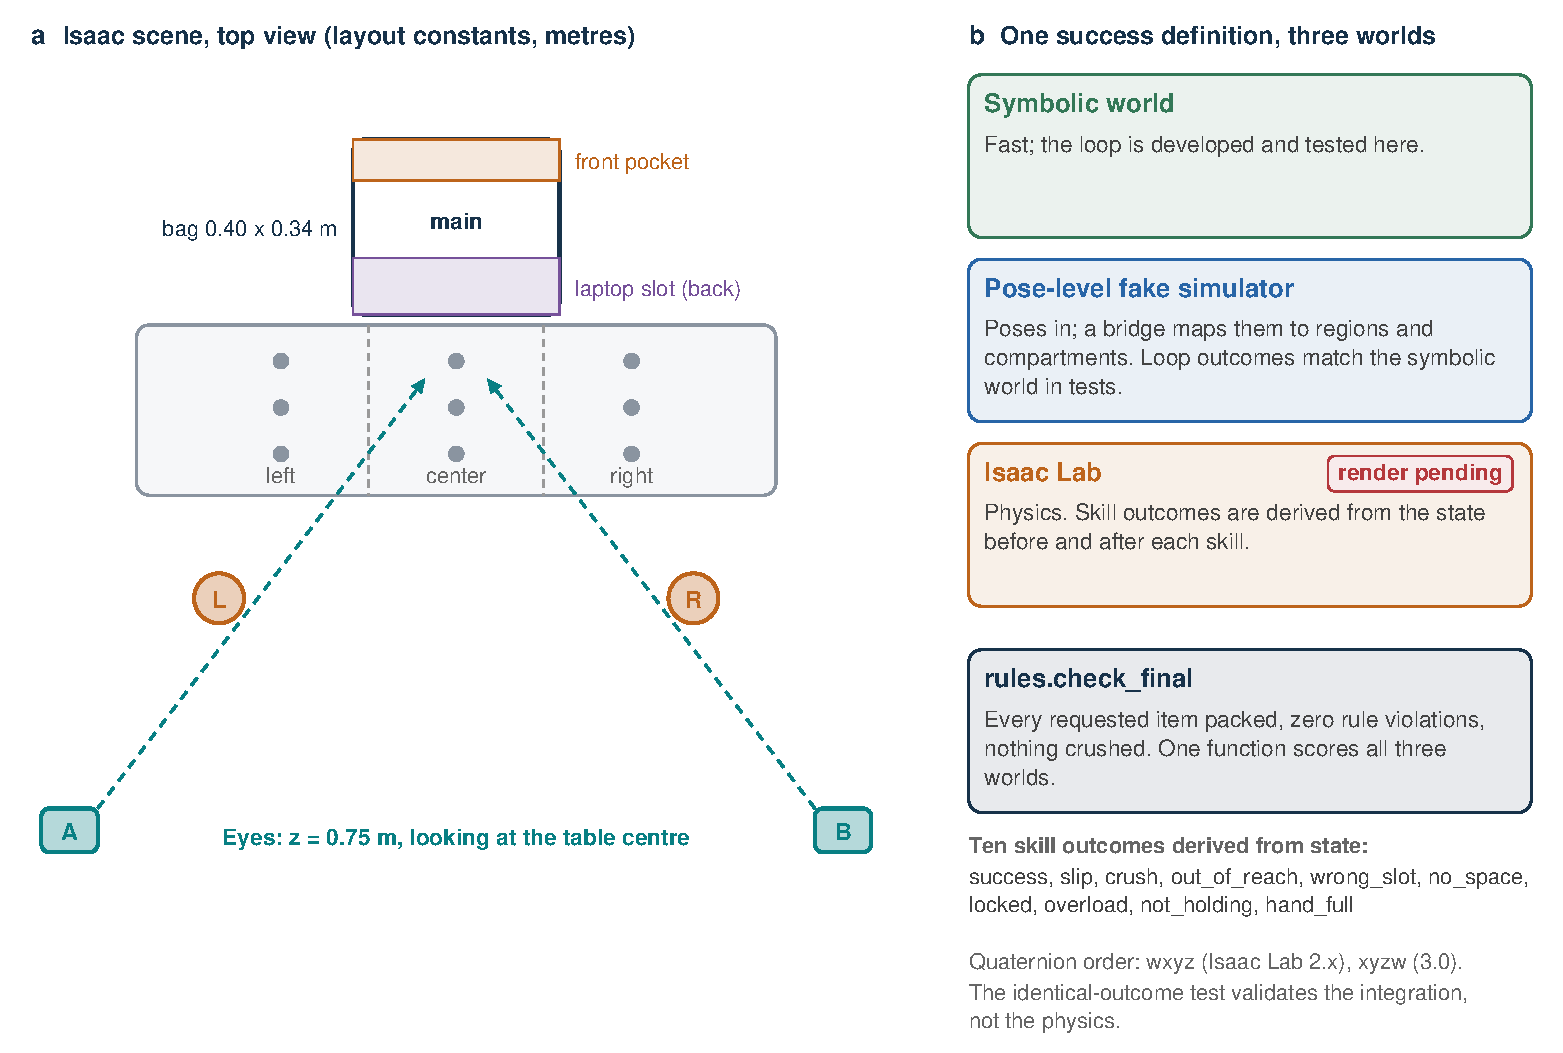
\includegraphics[width=\textwidth]{fig_bridge}
\caption{\textbf{The Isaac scene and the shared checker.} (a)~Top view from the layout constants: table zones, bag compartments, arm bases and camera positions. (b)~One success function scores three worlds. The Isaac render is pending.}
\label{fig:bridge}
\end{figure*}

\section{Evaluation protocol and status}\label{sec:experiments}

This section fixes the protocol before any trained result exists, so that the results cannot shape the questions.
\Cref{fig:design} is the planned design and \cref{tab:evidence} the status of each evidence class; every cell that no run has produced is a red flag.

\paragraph{Status of the evidence.}
The engineering gates G-1, G-2, G-3 and G-14 are measured and recorded in the repository; G-3 is a falling-cube rgb/depth gate on one device at a time and G-14 is a four-step resume smoke, not a task or model result. G-6 is a \emph{simulation-only} impedance cross-check (step error 0.27\,\%), not a hardware or safety result; G-6b measures the compliance supervisor on an abstract plant (SIM-ABSTRACT); and step A1 measures FR3 flange kinematics to within 0.00224\,mm over 102 configurations (\texttt{reports/g5\_reach.json}), a SIM-POSE, kinematics-only result.
\Cref{sec:gates} states each gate and where its report lives, and \cref{sec:matrix} states the held-out benchmark matrix; both are protocols until the corresponding reports exist.
\todo{No trained-model score, omni-model comparison, environment-trained Brain, arm certification or frontier-agent episode exists yet; the fixed fixture test set (seeds 0--29) has only a scripted-Brain score (\texttt{reports/test_scores.json}), not a model result, and the SimReady scene is not stepped. Every row below stays pending until a report exists. G-5, G-7 and G-13 are not run; A2--A10 and DG-1--DG-5 have no reports. Hardware safety sign-off is a separate future track (D-22); no hardware or human-safety result is claimed.}

\begin{figure*}[tbp]
\centering
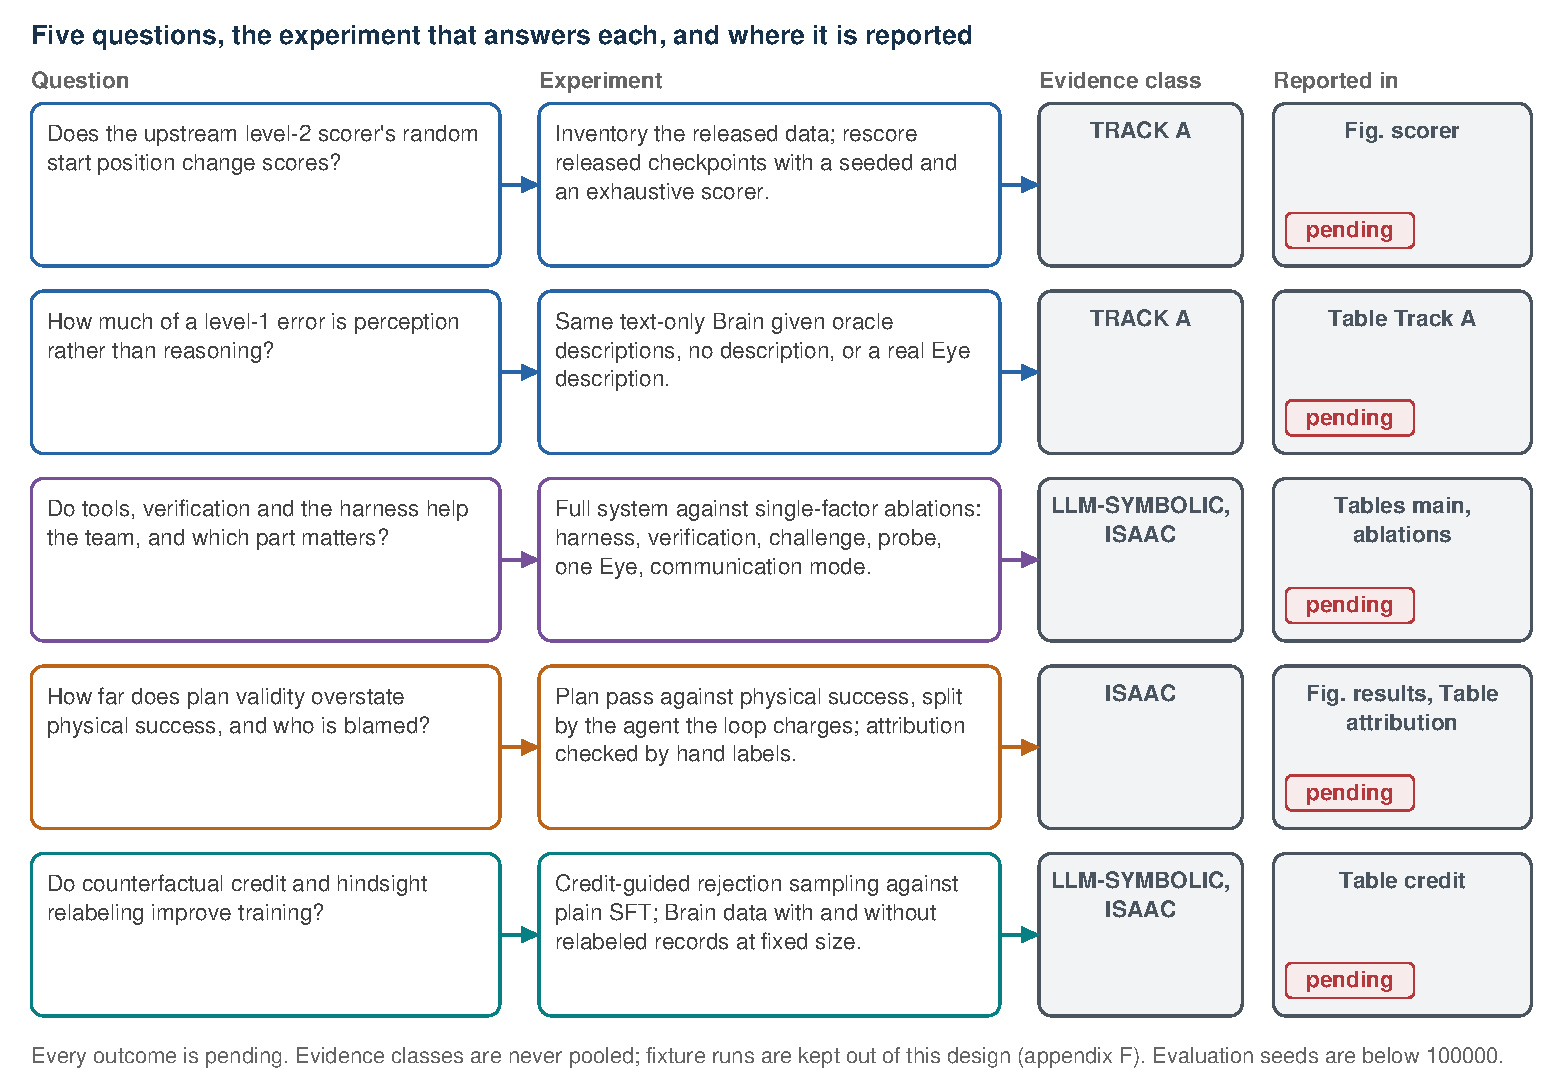
\includegraphics[width=0.95\textwidth]{fig_design}
\caption{\textbf{Planned evaluation design.} Five questions, the experiment that answers each, its evidence class and where it is reported. Track A uses real benchmark data and released models; Track B tests the packing team. Every outcome is pending, and fixture runs are kept out of the design (appendix~F).}
\label{fig:design}
\stalefig{the evidence-class column no longer matches what has actually been measured: the ISAAC class is drawn as if Isaac Lab manipulation episodes exist, whereas the only measured Newton evidence is the falling-cube rgb/depth gates G-3 (\texttt{reports/g3\_sim.json}, \texttt{reports/g3\_sim\_t4.json}), the simulation-only impedance cross-check G-6, the SIM-ABSTRACT compliance supervisor G-6b and the SIM-POSE A1 kinematics measurement. Split ISAAC into a GATE class (G-1/G-2/G-3/G-6/G-6b/A1/G-14, stating what each does and does not show) and a SIM/MODEL class (planned, not run); mark G-5, G-7, G-13, the arm runbook A1--A10 and the data-generation gates DG-1--DG-5 as not passed, mark the asset-based scene and scene bundle as not built, and keep ``every outcome is pending'' and the rule that classes are never pooled.}
\end{figure*}

\begin{table}[tbp]
\centering\small
\begin{tabular}{lp{0.3\linewidth}p{0.22\linewidth}l}
\toprule
Evidence class & What it is & Status in this version & Where reported \\
\midrule
TRACK A & Real VIKI-Bench data, real released models & \todo{pending} & \cref{tab:trackA} \\
ISAAC & Physics episodes in Isaac Lab & \todo{pending} & \cref{tab:main} \\
LLM-SYMBOLIC & A served LLM Brain on the symbolic task & \todo{pending} & \cref{tab:main,tab:ablations} \\
FIXTURE & Scripted Brain, flaky-planner wrapper, parametric Eyes & run (mechanism checks only) & \cref{app:fixture} \\
Engineering & Wiring tests on CPU with a tiny random model & run (proves wiring, not quality) & \cref{app:env} \\
\bottomrule
\end{tabular}

\caption{Evidence classes. A number is reported under exactly one class and never pooled with another.}
\label{tab:evidence}
\end{table}

\subsection{Protocol}\label{sec:protocol}
\paragraph{Evidence classes.}
TRACK~A is real VIKI-Bench data with real released models; ISAAC is physics episodes in Isaac Lab 3.0 with Newton (no Isaac Sim, no PhysX); LLM-SYMBOLIC is a served language-model Brain on the symbolic task; FIXTURE is a scripted Brain with a flaky-planner wrapper and parametric Eyes, used only to check mechanisms; engineering tests prove that code runs.
Each reported number carries its class.
\paragraph{Seeds and statistics.}
Training and data seeds are at least 100000 and evaluation seeds are below 100000, so no evaluation episode is in the training set.
Success rates are reported with Wilson 95\% intervals, and comparisons between conditions with paired bootstrap intervals over seeds; the claim a comparison supports is stated with its interval, never a bare rate.
Random draws are keyed so that conditions see the same episodes.
\paragraph{Compute.}
\todo{Compute is dual T4 GPUs on Kaggle (two 16\,GB cards), but the trainer and the G-3 scene step \emph{one device at a time}; no DDP training or two-GPU simulation exists (D-50, D-56). Confirm the memory plan for fine-tuning with fp16 LoRA without bf16, the model sizes that fit and the run times. Measured: the 4050 budget is 512 tokens for a forward/backward pass and 256 for SFT with adapters and optimizer state (D-38, D-47); the Newton-only stack passes G-3 on both the 4050 and a Kaggle T4 (D-39, D-51), where the rate is a JIT-warm-up artefact, not a throughput comparison.}

\subsection{Gates, not results}\label{sec:gates}
A gate is an engineering pass/fail criterion with a report under \texttt{reports/}; a measured gate is never pooled with a model-quality or hardware result, and a row without a report is not done.
\begin{itemize}[leftmargin=*,itemsep=1pt]
\item \textbf{Measured engineering gates.} G-1, the real Qwen3.5-4B module map (\texttt{reports/qwen35\_modules.json}); G-2, the DeltaNet fast path (\texttt{reports/g2\_fastpath.json}); G-3, Newton-only rgb/depth stepping on both the RTX~4050 and a Kaggle T4 (\texttt{reports/g3\_sim.json}, \texttt{reports/g3\_sim\_t4.json}) --- a falling cube, one device at a time, not manipulation; G-14, real-weight QLoRA SFT with a mid-epoch resume from our private repository (\texttt{reports/sft\_smoke.json}) --- a four-step smoke, not a trained model.
\item \textbf{Compliance and kinematics, by evidence class.} G-6 is a simulation-only impedance cross-check (\texttt{reports/g6\_impedance.json}); G-6b measures the compliance supervisor on a SIM-ABSTRACT point mass (\texttt{reports/g6b\_compliance.json}); step A1 measures FR3 flange forward kinematics against Newton to 0.00224\,mm over 102 configurations (\texttt{reports/g5\_reach.json}), SIM-POSE and kinematics only. None is a safety certification.
\item \textbf{Arm gates, not passed.} G-5 covers loading the FR3/FR3 Duo and Franka Hand in Newton with an effort-mode override (\texttt{reports/g5\_fr3.json}); G-7 covers external wrench injection with multiple solver substeps (\texttt{reports/g7\_wrench.json}); G-13 covers SimReady ingestion into Newton (\texttt{reports/g13\_usd\_ingest.json}, partial); the arms-first runbook A1--A10 ends in certification cards and outcome tables (\texttt{reports/arm\_cert\_*.json}, \texttt{skill\_tables/manifest.json}). \todo{No manipulation, push or arm-certification report exists; only the A1 kinematics half of G-5 is measured. Hardware/L0/L1 sign-off is assigned to a separate future track (D-22).}
\item \textbf{Data-generation gates, not passed.} DG-1--DG-5 cover the hosted Haiku run, the GPU-kernel roster, replay of real records, the first memory iteration and an image turn (design and cost estimates in the Kaggle data-generation notes). \todo{The hosted loop is built and fixture-tested on SIM-POSE; no Kaggle endpoint has been called and no frontier model has run.}
\end{itemize}

\subsection{Held-out benchmark matrix}\label{sec:matrix}
The held-out test set uses seeds below 100000 exclusively, with at least 30 episodes per family: packing variants, heavy/fragile ordering, occlusion-heavy arrangements, distractors, handover-required cases, human-push interruption, kitchen tasks on SimReady objects, and unseen layouts and objects.
The matrix is exact (D-64): M1, base Qwen3.5-4B zero-shot; M2, base Qwen3.5-9B zero-shot; M3, 4B SFT; M4, 4B SFT with GRPO at $k=4$; M5, 4B SFT with GRPO at $k=8$; M6, frontier models zero-shot; M7, the same frontier models in the harness (skills, tools, memory, rules and success/failure-memory retrieval); M8, base 4B in the harness.
The isolated effects are SFT (M3 minus M1), GRPO at $k=4$ and $k=8$ (M4 and M5 minus M3), the harness on frontier models (M7 minus M6) and on the base 4B (M8 minus M1).
Metrics include success, plan pass, per-family success, localisation, occlusion handling, eye-tool use, two-arm coordination, recovery, collisions and compliance (push deflection, settle time, return speed and plan-pause correctness), each with Wilson intervals and paired bootstrap over seeds; every cell traces to a run card carrying a config hash, seed list and model revision.
\todo{This matrix is a protocol only: no row has a measured number, and the frontier rows in eval mode have not been run.}

\subsection{Track A: real benchmark data and released models}\label{sec:track-a}
Track A re-evaluates the released VIKI-R checkpoints on VIKI-Bench with our own runner, and decomposes a level-1 error into perception and reasoning by giving a text-only Brain oracle descriptions, no description, or a real Eye description of the same image (\cref{tab:trackA}).
If compute allows, a matched-base control trains the same base model with the upstream recipe, so that any difference from our additions is attributable.
\todo{Pin the upstream VIKI-R repository commit and dataset revision; record licences.}

\begin{table}[tbp]
\centering\small
\begin{tabular}{p{0.40\linewidth}cccc}
\toprule
Condition & L1 accuracy & L2 accuracy & Format rate & Failed items \\
\midrule
Released VIKI-R checkpoints, upstream-style scoring & \todo{pending} & \todo{pending} & \todo{pending} & \todo{pending} \\
Released checkpoints, position-robust scoring, full split & \todo{pending} & \todo{pending} & \todo{pending} & \todo{pending} \\
Text-only Brain with oracle descriptions & \todo{pending} & \todo{pending} & \todo{pending} & \todo{pending} \\
Same Brain, no Eye description & \todo{pending} & \todo{pending} & \todo{pending} & \todo{pending} \\
Same Brain, real Eye description & \todo{pending} & \todo{pending} & \todo{pending} & \todo{pending} \\
Matched-base control (Qwen2.5-VL-3B), if compute allows & \todo{pending} & \todo{pending} & \todo{pending} & \todo{pending} \\
\bottomrule
\end{tabular}

\caption{Track A design. L1 and L2 are VIKI-Bench levels. All cells are pending.}
\label{tab:trackA}
\end{table}

\subsection{An audit of the upstream level-2 scorer}\label{sec:scorer}
We read the upstream level-2 scoring code.
It checks a plan with a pure-Python feasibility function, so no simulator is involved; for each asset it draws a start position with \texttt{random.choice} on every call, and a plan counts as correct if it is feasible and the ratio of reference length to plan length is at least 0.99; the reward is 0.1 for format plus 0.9 for correctness.
The evaluation scripts read only the first 900 level-2 rows and the first 1000 level-1 rows, and the level-2 script loads one split file but writes to a directory with another name.
\Cref{fig:scorer} shows the consequence on a toy case we built: if a plan is valid only for some start positions, an unseeded scorer passes it by luck of the draw.
In the toy case, 40 unseeded draws pass 18 times, the exhaustive average over start positions is 0.5, and a position-agnostic plan passes 40 of 40.
This is a synthetic demonstration of the mechanism; how many real VIKI-Bench items depend on a random start position is unknown until the inventory script runs on the dataset, and we make no claim about the published numbers.
\todo{Run the inventory on the released data; report the fraction of items affected, and rescore the released checkpoints with a seeded and an exhaustive scorer.}

\begin{figure*}[tbp]
\centering
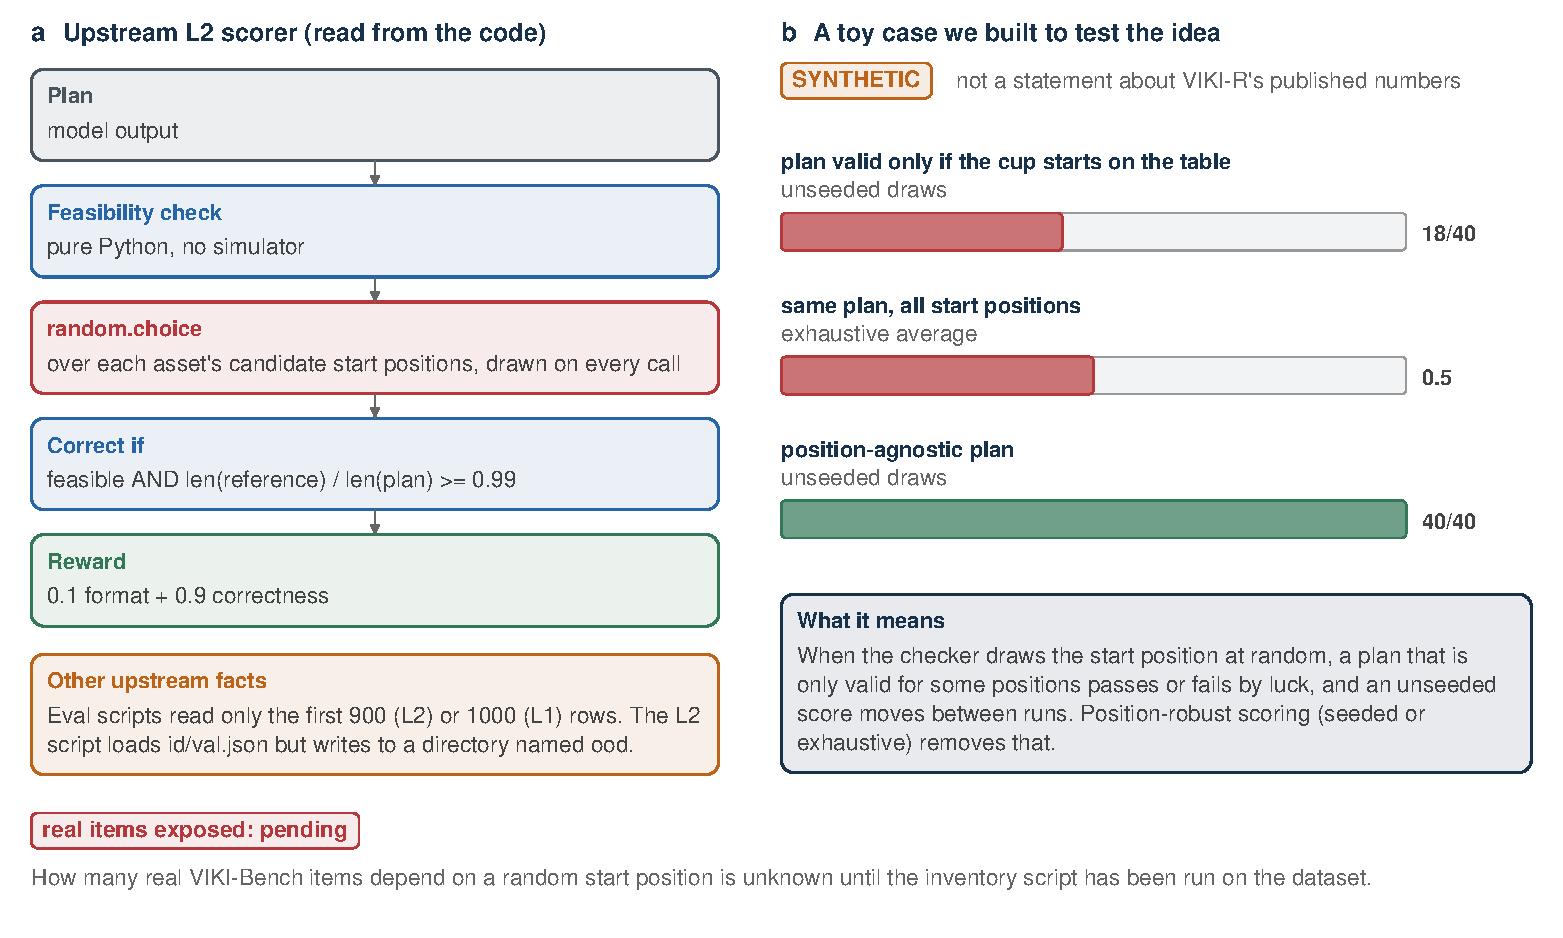
\includegraphics[width=\textwidth]{fig_scorer_audit}
\caption{\textbf{Audit of the upstream level-2 scorer.} (a)~The scoring path as read from the code; the highlighted step draws start positions at random on every call. (b)~A synthetic toy case: a plan valid only for some start positions passes 18 of 40 unseeded draws, has an exhaustive average of 0.5, and a position-agnostic plan passes 40 of 40. The toy case is not a statement about the published VIKI-R numbers.}
\label{fig:scorer}
\end{figure*}

\subsection{Track B: the packing team}\label{sec:track-b}
Track B runs the team on procedurally generated packing tasks, in the symbolic world with a served Brain (LLM-SYMBOLIC) and in Isaac Lab (ISAAC) (\cref{tab:main}).
The headline measurement is the gap between plan validity and physical success: the fraction of episodes whose plan passes the dry run but whose physical episode fails, split by the agent the loop charges.
\Cref{fig:results} draws the results from the results bundle when one exists, and is otherwise a red placeholder.

\begin{table}[tbp]
\centering\small
\begin{tabular}{p{0.36\linewidth}cccc}
\toprule
Condition (Track B, one evidence class per run) & Success [95\% Wilson] & Plan pass & Replans & Msg tokens \\
\midrule
Full system, LLM-SYMBOLIC & \todo{pending} & \todo{pending} & \todo{pending} & \todo{pending} \\
Full system, ISAAC & \todo{pending} & \todo{pending} & \todo{pending} & \todo{pending} \\
\bottomrule
\end{tabular}

\caption{Track B main results (pending). Success with a Wilson interval, the fraction of plans passing the dry run, replans per episode and message tokens.}
\label{tab:main}
\end{table}

\begin{figure*}[tbp]
\centering
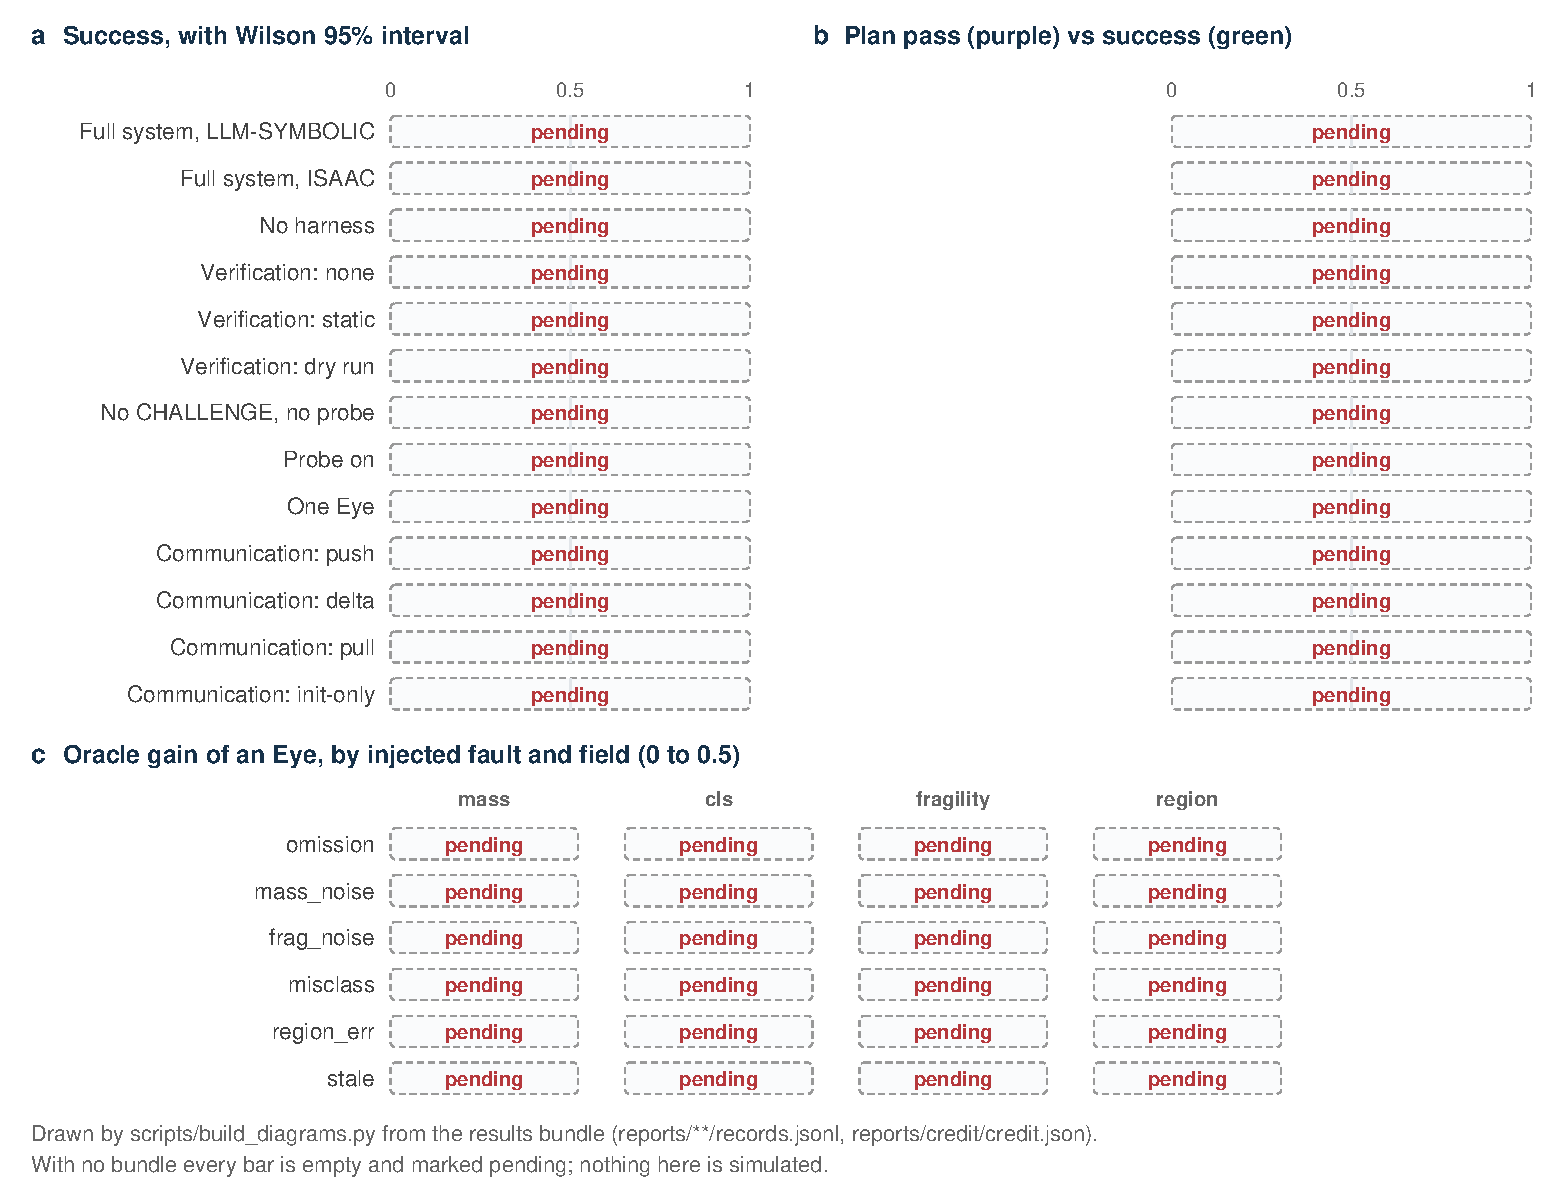
\includegraphics[width=0.95\textwidth]{fig_results}
\caption{\textbf{Results figure, generated from the results bundle.} (a)~Success per configuration with Wilson intervals. (b)~Plan pass against success. (c)~Oracle gain by injected fault and field. With no bundle present every bar is empty and marked pending; nothing here is simulated.}
\label{fig:results}
\end{figure*}

\subsection{Ablations}\label{sec:ablations}
\Cref{tab:ablations} lists the ablations: the harness, the three verification modes, challenge and probe, one Eye against two, and the four communication modes.
Each is a code configuration, so the comparison differs in one factor.
\begin{table}[tbp]
\centering\small
\begin{tabular}{p{0.36\linewidth}cccc}
\toprule
Ablation & Success [95\% Wilson] & Plan pass & Replans & Msg tokens \\
\midrule
No harness & \todo{pending} & \todo{pending} & \todo{pending} & \todo{pending} \\
Verification: none & \todo{pending} & \todo{pending} & \todo{pending} & \todo{pending} \\
Verification: static & \todo{pending} & \todo{pending} & \todo{pending} & \todo{pending} \\
Verification: dry run & \todo{pending} & \todo{pending} & \todo{pending} & \todo{pending} \\
No CHALLENGE, no probe & \todo{pending} & \todo{pending} & \todo{pending} & \todo{pending} \\
Probe on & \todo{pending} & \todo{pending} & \todo{pending} & \todo{pending} \\
One Eye & \todo{pending} & \todo{pending} & \todo{pending} & \todo{pending} \\
Communication: push & \todo{pending} & \todo{pending} & \todo{pending} & \todo{pending} \\
Communication: delta & \todo{pending} & \todo{pending} & \todo{pending} & \todo{pending} \\
Communication: pull & \todo{pending} & \todo{pending} & \todo{pending} & \todo{pending} \\
Communication: init-only & \todo{pending} & \todo{pending} & \todo{pending} & \todo{pending} \\
\bottomrule
\end{tabular}

\caption{Ablations (pending).}
\label{tab:ablations}
\end{table}

\subsection{Counterfactual credit and hindsight}\label{sec:credit-eval}
We evaluate the credit signal on whether rejection sampling guided by it produces Eyes with a smaller oracle gain than plain fine-tuning, and report the gain with its field breakdown (\cref{tab:credit}).
The fixture version of the credit estimate, which checks that the estimator recovers the injected fault, is in appendix~F.
For hindsight relabeling we compare Brain training with and without relabeled records at fixed total size.
\begin{table}[tbp]
\centering\small
\begin{tabular}{p{0.28\linewidth}ccccc}
\toprule
Eye variant & Oracle gain G & mass & class & fragility & region \\
\midrule
Plain SFT Eye & \todo{pending} & \todo{pending} & \todo{pending} & \todo{pending} & \todo{pending} \\
Rejection-sampled Eye & \todo{pending} & \todo{pending} & \todo{pending} & \todo{pending} & \todo{pending} \\
Fixed-Brain counterfactual & \todo{pending} & \todo{pending} & \todo{pending} & \todo{pending} & \todo{pending} \\
\bottomrule
\end{tabular}

\caption{Oracle gain $G$ of trained Eyes and its breakdown by field (pending).}
\label{tab:credit}
\end{table}

\subsection{Is the attribution right?}\label{sec:attribution-eval}
The attribution rules are heuristics, so we check them against hand labels on a sample of failed episodes and report agreement and Cohen's $\kappa$ per agent (\cref{tab:attribution}).
\todo{Choose the number of episodes to hand-label and who labels them.}
\begin{table}[tbp]
\centering\small
\begin{tabular}{lccc}
\toprule
Agent label & Episodes labelled by hand & Agreement with the heuristic & Cohen's kappa \\
\midrule
Eye & \todo{pending} & \todo{pending} & \todo{pending} \\
Brain & \todo{pending} & \todo{pending} & \todo{pending} \\
Arm & \todo{pending} & \todo{pending} & \todo{pending} \\
\bottomrule
\end{tabular}

\caption{Agreement of the loop's attribution with hand labels (pending).}
\label{tab:attribution}
\end{table}

\section{Limitations}\label{sec:limits}
\begin{itemize}[leftmargin=*,itemsep=1pt]
\item \textbf{No trained-model result.} All trained-model, benchmark and physics numbers are pending; the mechanism evidence comes from a symbolic fixture with a scripted Brain and parametric Eyes (FIXTURE), and the asset-backed traces and memory are pose-level (SIM-POSE). Neither says anything about a trained agent.
\item \textbf{Hosted tasks are CPU-only, without torch.} The Newton scene cannot run inside a Kaggle hosted task, so frontier episodes are served from a scene bundle of cached views and sampled certified outcomes. A CPU episode is only as faithful as that bundle's agreement with a direct Newton replay, a tolerance we have not measured; the GPU replay gate is not built.
\item \textbf{Kaggle access is not yet available to us.} Calling the hosted frontier models depends on a user-supplied model catalogue, CLI authorisation and the local proxy; no frontier endpoint has been called, and all chain-of-thought traces to date come from a scripted teacher. Cost and yield figures are estimates.
\item \textbf{Asset ingestion is partial.} Only a subset of the SimReady USD packages imports cleanly into Newton; G-13 is not passed, there are no drop, grasp or texture-contract results, and the assembled asset-based scene has not been stepped or rendered. The scene bundle and view library do not exist.
\item \textbf{Arm certification is not built.} The arms-first runbook A1--A10 has not run: the only arm measurement is the A1 flange kinematics agreement (SIM-POSE, kinematics only), the compliance supervisor is measured on an abstract plant (SIM-ABSTRACT), and there are no results on the Newton articulation, no push-perturbed evaluation and no certification cards or outcome tables. The claim that data generation is gated on certified arms is therefore a design decision, not a demonstrated pipeline.
\item \textbf{Simulation is not safety, and there are no hardware results.} Impedance and compliant yielding are measured control behaviours, not a safety certification; force, speed and contact caps remain placeholders until the applicable standard is read. Hardware safety sign-off is assigned to a separate future track (D-22), and we make no claim that the arms are safe around people or children.
\item \textbf{The scorer demonstration is synthetic.} We show that a random start-position draw can make a score depend on luck in a toy case; we do not know how many real items are affected.
\item \textbf{Attribution is heuristic.} The labels are rules over reported and true quantities, not ground truth about causes, until \cref{tab:attribution} is filled.
\item \textbf{Counterfactual credit is a team estimate.} It is not additive across redundant Eyes, and with an adaptive Brain it measures the adapted team.
\item \textbf{Small, procedural task.} Backpack packing with six rules in simulation says little about open-ended manipulation, and no real robot is involved.
\item \textbf{Pose-level agreement is not physics.} The identical-outcome test validates the integration of the bridge, not the physical behaviour.
\item \textbf{Teacher plans.} Brain fine-tuning data would come from hosted frontier models (or, so far, a scripted teacher), so the Brain may inherit their biases; no verified corpus exists yet.
\item \textbf{Related work is incomplete.} Several multi-agent embodied systems named in our plan have not been read and are not compared; see \cref{sec:related}.
\item \textbf{Compute.} \todo{State the effect of the dual-T4 budget on model size, training length and the physics track once confirmed: the trainer and the G-3 scene step one device at a time, and no DDP or two-GPU simulation exists (D-50, D-56).}
\end{itemize}

\section{Conclusion}\label{sec:conclusion}
We described a two-arm kitchen-packing team whose ordering constraint is to certify the compliant arms before any language-model data generation: an impedance and compliance supervisor provides push, yield, return and resume behaviour, and the Brain emits only skills and eye commands, never joints, gains or speeds.
Around that substrate we placed two movable eyes with a rendered view library and tool surface, a scene bundle of SimReady USD assets and measured arm outcome tables, a hosted multi-turn data loop that captures every frontier-model turn and replay-verifies it into a success/failure memory and a per-model ledger, and a training path of SFT and GRPO at $k=4$ and $k=8$ scored on the held-out M1--M8 matrix.
The interface separation also makes failures attributable, and we specified two training signals that follow from it: counterfactual Eye credit and team hindsight relabeling with a replay check.
An audit of the upstream level-2 scorer shows, on a synthetic case, how random start positions can make scores depend on luck.
The system architecture and evaluation protocol are fixed, and engineering gates and evidence classes are reported separately; every arm-certification, data-generation, trained-model, benchmark and hardware result is pending, and we make no safety claim about the arms (D-22).
The next step is to run the arms-first runbook and the Kaggle data gates, then to fill \cref{tab:trackA,tab:main,tab:ablations,tab:credit,tab:attribution} and the matrix of \cref{sec:matrix}, reporting each row under its own evidence class.


\section*{Data and code availability}
\todo{Add repository, Hub and DOI links before submission.} The figure and table scripts in \texttt{scripts/} regenerate every figure and number in this paper from recorded data (\cref{app:repro}).

\FloatBarrier
\bibliographystyle{plainnat}
\bibliography{refs}

\appendix
\section{Message schema}\label{app:messages}
\Cref{tab:messages} in \cref{sec:bus} lists the \nMsgTypes{} message types with their required fields as implemented; the bus rejects a message that lacks a required field and charges tokens at about four characters per token.

\section{Harness files}\label{app:harness}
\begin{table}[h]
\centering\scriptsize
\begin{tabular}{llp{0.5\linewidth}}
\toprule
File & Type & Retrieval keywords \\
\midrule
\texttt{agents/arm\_L.md} & agent & left arm L reach table\_left table\_center \\
\texttt{agents/arm\_R.md} & agent & right arm R reach table\_right table\_center \\
\texttt{agents/eye.md} & agent & eye camera scene report occlusion \\
\texttt{memory/episodes.md} & memory & episodic memory past failures lessons \\
\texttt{objects/book.md} & object & book textbook heavy robust \\
\texttt{objects/bottle.md} & object & bottle water liquid upright \\
\texttt{objects/laptop.md} & object & laptop heavy fragile notebook computer \\
\texttt{objects/lunchbox.md} & object & lunchbox food container \\
\texttt{rules/bag\_exclusive.md} & rule & bag opening exclusive lock one arm at a time \\
\texttt{rules/bottle\_upright.md} & rule & bottle water upright away laptop leak \\
\texttt{rules/heavy\_bottom.md} & rule & heavy bottom stack order weight mass main compartment \\
\texttt{rules/laptop\_slot.md} & rule & laptop padded slot compartment protect \\
\texttt{rules/leave\_distractors.md} & rule & leave distractor mug plate untouched not pack \\
\texttt{rules/lunchbox\_last.md} & rule & lunchbox last final order top \\
\texttt{skills/grasp.md} & skill & grasp force slip crush payload \\
\texttt{skills/handover.md} & skill & handover transfer arm center \\
\texttt{skills/place.md} & skill & place compartment orientation insert bag capacity \\
\texttt{skills/push\_aside.md} & skill & push aside clear occlusion \\
\texttt{tasks/pack\_backpack.md} & task & pack backpack school bag items instruction \\
\bottomrule
\end{tabular}

\caption{The \nHarnessFiles{} harness files with their retrieval keywords.}
\end{table}

\section{Reward and score definitions}\label{app:rewards}
\paragraph{Brain plan reward.} $R = 0.1\,r_{\text{format}} + 0.2\,r_{\text{feasible}} + 0.6\,r_{\text{rules}} + 0.1\,r_{\text{length}}$ with an optional closed-loop rollout term of weight 0.5.
$r_{\text{format}}$ checks that the output parses as a plan; $r_{\text{feasible}}$ is 1 if the static check passes and otherwise falls with the fraction of erroneous tasks; $r_{\text{rules}}$ is the valid-item fraction from a deterministic dry run minus 0.25 per rule violation and per crush, floored at 0; $r_{\text{length}}$ is 1 up to 24 tasks and falls linearly to 0 at 48.
\paragraph{Episode score.} The valid-item fraction minus 0.15 per violation, 0.3 per crushed item and 0.01 per replan.
\paragraph{Credit.} $C(i,r)=R(\text{real})-R(i,r)$; oracle gain $G=-C(i,\text{oracle})$ (\cref{sec:signals}).

\section{Upstream facts and the scorer toy case}\label{app:viki}
The scorer facts in \cref{sec:scorer} were read from the upstream VIKI-R repository by the authors: simulator-free feasibility check, \texttt{random.choice} over each asset's candidate start positions on every call, correctness as feasible and length ratio at least 0.99, reward 0.1 format plus 0.9 correctness, evaluation scripts reading the first 900 level-2 and 1000 level-1 rows, and the level-2 script reading one split file while writing to a directory with another name.
\todo{Pin the repository commit; re-run the toy case (18 of 40 unseeded draws, exhaustive average 0.5, position-agnostic plan 40 of 40) against the upstream scorer. The toy numbers are from an earlier run by the authors and could not be re-run in this build because the upstream code was not available to it, which also left the scorer tests skipped.}

\section{Environment and tests}\label{app:env}
The code base is a Python package with a symbolic world, a pose-level simulator, the loop, the harness and training scripts; the physics stack is Isaac Lab 3.0 with Newton (\texttt{mujoco-warp}), with no Isaac Sim and no PhysX, and that configuration was measured on the RTX 4050 and on a Kaggle T4 (gate G-3: 30 steps, rgb and depth contracts, D-39 and D-51), stepping one device at a time (D-50).
In the training environment (Python 3.12, torch 2.15, transformers 5.23) the test suite passes with the unavailable upstream VIKI-R clone tests skipped, so the scorer tests do not run in a clean build.
This proves that the code runs and that the wiring is consistent, and is not evidence about model quality.
\todo{Quote the current passed/skipped count from the gate record at submission time; earlier figures here, including the CPU-only 137/13 baseline, are superseded by the measured training-venv count.}

\section{Fixture mechanics checks}\label{app:fixture}
All runs here are class FIXTURE: a symbolic world, a scripted Brain, parametric Eyes and a flaky-planner wrapper, seeds 0 to \fxN{} minus one.
They check that mechanisms behave as designed and are not claims about trained agents.
The numbers come from \texttt{scripts/collect\_fixture.py}.

\begin{table}[h]
\centering\small
\begin{tabular}{lccc}
\toprule
Verification & Successes & Wilson 95\% & Retries used \\
\midrule
none & 48/80 & [0.49, 0.70] & 0 \\
static & 63/80 & [0.69, 0.86] & 29 \\
dry run & 80/80 & [0.95, 1.00] & 48 \\
dry run, 0 retries & 48/80 & [0.49, 0.70] & 0 \\
\bottomrule
\end{tabular}

\caption{Plan verification against a planner wrapped to inject errors with probability 0.5 (clean Eyes).}
\end{table}
\begin{table}[h]
\centering\small
\begin{tabular}{lcc}
\toprule
Mode & Successes & Message tokens per episode \\
\midrule
push & 73/80 & 10{,}551 \\
delta & 73/80 & 5{,}737 \\
pull & 72/80 & 1{,}895 \\
init-only & 71/80 & 1{,}182 \\
\bottomrule
\end{tabular}

\caption{Communication modes (noisy Eyes): message tokens are a four-characters-per-token proxy.}
\end{table}
\begin{table}[h]
\centering\small
\begin{tabular}{lccc}
\toprule
Condition & Successes & Wilson 95\% & Mean rounds \\
\midrule
probe & 80/80 & [0.95, 1.00] & 16.56 \\
challenge only & 39/80 & [0.38, 0.60] & 14.00 \\
no fix & 22/80 & [0.19, 0.38] & 14.35 \\
\bottomrule
\end{tabular}

\caption{Heavy Eye mass noise ($\sigma=0.45$ on both Eyes): weighing probe, challenge only, and no fix.}
\end{table}
\begin{table}[h]
\centering\small
\begin{tabular}{lcc}
\toprule
Eyes (omission fault) & LOOK off & LOOK on \\
\midrule
1 & 1/80 & 48/80 \\
2 & 15/80 & 75/80 \\
\bottomrule
\end{tabular}

\caption{Effect of the look request when each Eye omits an item with probability 0.4.}
\end{table}
\begin{table}[h]
\centering\small
\begin{tabular}{lcccccc}
\toprule
Eye fault & Mean episode score & Oracle gain G [95\% CI] & mass & class & fragility & region \\
\midrule
omission & 0.992 & 0.008 [0.002, 0.016] & 0.000 & 0.000 & 0.000 & 0.000 \\
mass\_noise & 0.826 & 0.174 [0.131, 0.223] & 0.174 & 0.000 & 0.000 & 0.000 \\
frag\_noise & 0.999 & 0.001 [0.000, 0.001] & 0.000 & 0.000 & 0.001 & 0.000 \\
misclass & 0.905 & 0.095 [0.056, 0.139] & 0.000 & 0.095 & 0.000 & 0.000 \\
region\_err & 0.954 & 0.046 [0.031, 0.062] & 0.000 & 0.000 & 0.000 & 0.046 \\
stale & 0.880 & 0.120 [0.091, 0.151] & 0.120 & 0.000 & 0.000 & 0.000 \\
\bottomrule
\end{tabular}

\caption{Oracle gain $G$ for Eye~A by injected fault type, with the breakdown by field: the estimator puts the gain in the field that carries the fault.}
\end{table}

\section{Reproducing the figures and numbers}\label{app:repro}
\begin{table}[h]
\centering\small
\begin{tabular}{lp{0.62\linewidth}}
\toprule
Item & Value \\
\midrule
Training and data seeds & $\geq 100000$ \\
Evaluation seeds & $< 100000$ \\
Stochastic draws & keyed by (seed, arm, skill, object, attempt); Eye noise by (seed, eye, time) \\
Python / simulator & 3.12 / Isaac Lab 3.0 with Newton (no Isaac Sim, no PhysX) \\
Compute & RTX 4050 (6 GB, dev) and Kaggle dual T4; G-3 PASS on both GPU classes, one device at a time (D-39, D-51) \\
Code and data release & \todo{repository, Hub and DOI links} \\
\bottomrule
\end{tabular}

\caption{Reproducibility facts.}
\end{table}
\begin{small}
\begin{verbatim}
python scripts/collect_figdata.py --project ../robot_team
python scripts/collect_fixture.py --project ../robot_team
python scripts/build_diagrams.py     # 12 figures, SVG + PDF
python scripts/audit_diagram_text.py; python scripts/audit_diagram_arrows.py
python scripts/build_paper.py        # tables, number macros, pending lists
python scripts/verify_paper.py       # numbers, citations, pending cells
pdflatex main; bibtex main; pdflatex main; pdflatex main
\end{verbatim}
\end{small}


\end{document}
